\documentclass[mathserif]{beamer}
\usepackage{beamerthemeshadow}
\usepackage{beamerthemesplit}
%\usetheme{shadow}
\usecolortheme{default}
\setbeamertemplate{footline}[frame number]
\useinnertheme[shadow=true]{rounded}
%\setbeamertemplate{footline}{\insertframenumber/\inserttotalframenumber}
%\useoutertheme{infolines}
%\setbeamertemplate{headline}{} % removes the headline that infolines inserts

%\usetheme{boxes}
%\usepackage{amsmass}
%\usepackage{amssymb,amsfonts,url}

\usepackage{algorithm}
\usepackage{algorithmic}

\usepackage{graphicx}
\graphicspath{{Problems/}}

%\usepackage{CJK}
%\usepackage{pinyin}

%    \begin{figure}
%        \centering
%        \includegraphics[width=0.8\textwidth]{newGeneRep.eps}
%    \end{figure}

% \begin{figure}%
%   \begin{center}%
%     \begin{minipage}{0.70\textwidth}%
%      \includegraphics[width=1.0\textwidth]{comp25000.eps}%
%     \end{minipage}%
%     \begin{minipage}{0.30\textwidth}
%      \includegraphics[width=1.0\textwidth]{comparelabel.eps}%
%     \end{minipage}%
%   \end{center}
% \end{figure}

% \begin{table}
%   {\begin{tabular}{l|rrr}\hline
%       & \multicolumn{3}{c}{Actual number of DCJ operations}\\
%       \# genes &\# genes $\times 1$&\# genes $\times 2$&\# genes  $\times 3$ \\
% \hline
%      (a)~25,000 & 0.5\% ~~&  0.9\% ~~& 1.7\%~~\\
%       (b)~10,000 & 0.8\%~~ &  1.4\% ~~& 2.7\%~~\\
%      (c)~ 1,000 & 2.7\%~~ & 4.7\%~~ & 14.7\%~~\\ \hline
%     \end{tabular}} {}%
% \end{table}

% \begin{eqnarray}
% T(n) &=&  \sum\nolimits_{i=1}^n C_i \\
%      &=&  \# PUSH + \#POP \\
%      &<& 2\times \#PUSH \\
%      &<& 2n \\
% \end{eqnarray}

% \[ 
% \begin{matrix}
% \begin{pmatrix}
% C_{11} & C_{12} \\ 
% C_{21} & C_{22} 
% \end{pmatrix}
% =
% \begin{pmatrix}
% A_{11} & A_{12} \\ 
% A_{21} & A_{22}  
% \end{pmatrix}
% 
% \begin{pmatrix}
% B_{11} & B_{12} \\ 
% B_{21} & B_{22}  
%  
% \end{pmatrix}
%     
%    \end{matrix}
% \]
% 
% 
% \begin{eqnarray}
%  C_{11} &=& (A_{11}\times B_{11}) + (A_{12} \times B_{21}) \\
% C_{12} &=& (A_{11}\times B_{12}) + (A_{12} \times B_{22}) \\
% C_{21} &=& (A_{21}\times B_{11}) + (A_{22} \times B_{21}) \\
% C_{22} &=& (A_{21}\times B_{12}) + (A_{22} \times B_{22}) 
% \end{eqnarray}
% \begin{figure}%
%      \begin{minipage}{0.32\textwidth}%
%       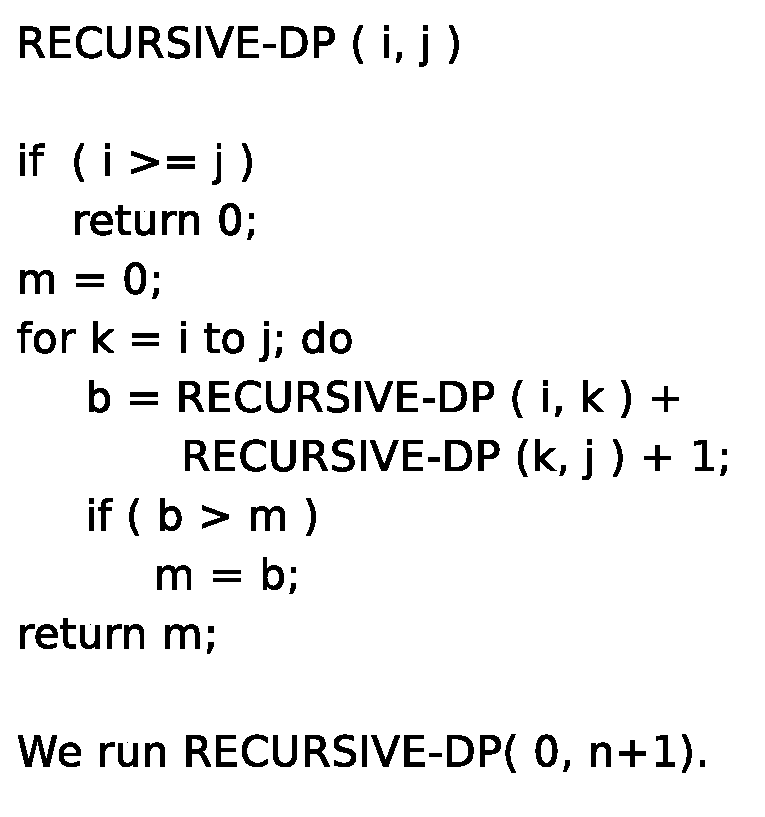
\includegraphics[width=1.0\textwidth]{L7-intervalschedulingdpalgo.eps}%
%      \end{minipage}%
%  \quad
%      \begin{minipage}{0.30\textwidth}
%       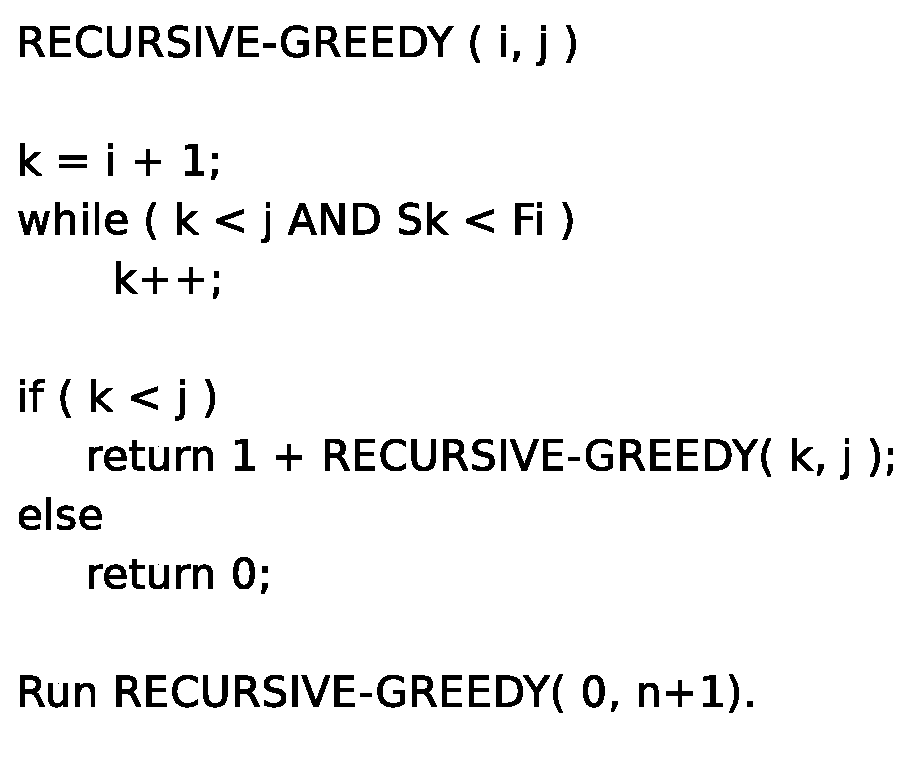
\includegraphics[width=1.0\textwidth]{L7-intervalschedulinggreedyalgo.eps}%
%      \end{minipage}%
%  \quad
%       \begin{minipage}{0.25\textwidth}
%       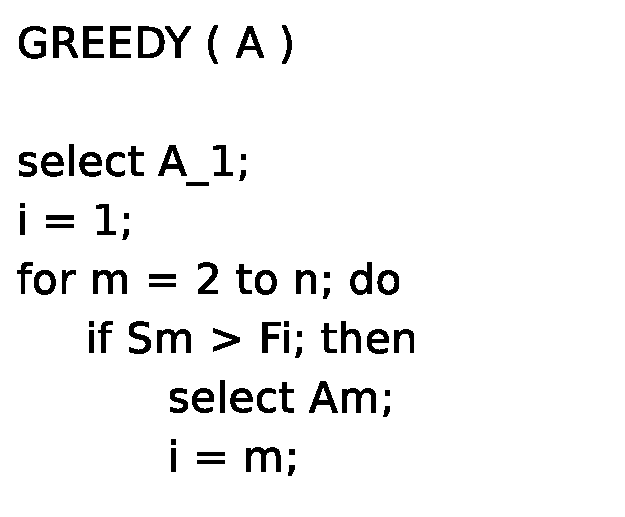
\includegraphics[width=1.0\textwidth]{L7-intervalschedulinggreedyalgo2.eps}%
%      \end{minipage}%
% 
%  \end{figure}

\title{CS612  Algorithm Design and Analysis }
\subtitle{ Lecture 13. Extending the limits of tractability 
%\footnote{The slides are made based on Chapter 10 of Algorithm design, and lectures by D. P. Williamson. } 
}
\author{Dongbo Bu } 
\institute{ {\small Institute of Computing Technology \\ 
Chinese Academy of Sciences, Beijing, China}}

\date{}

\begin{document}
%\begin{CJK}{UTF8}{cyberbit}

\frame[allowframebreaks]{\titlepage}

\frame{
\frametitle{Outline}
\begin{itemize}
\item Introduction to FPT(Fixed parameter tractability) problems;
\item Solving special cases of NP-Hard problems:
\begin{enumerate}
\item Solving a problem when \textcolor{red}{parameters are small}: {\sc VertexCover};
\item Solving a problem when \textcolor{red}{connection among sub-problems is small}: 
\begin{itemize}
\item NP-Hard problems might be easy when input is a \textcolor{red}{tree}: {\sc IndependentSet}, and {\sc WeightedIndependentSet};
\item Extending tree to tree-like: tree-decomposition of graph;  
\end{itemize}
\end{enumerate} 
\end{itemize}

Note: 
\begin{itemize}
\item \textcolor{red}{ A particular practical instance of a NP-Hard problem might has special structure to make it easier than the worst cases.}
\item \textcolor{red}{If we have an efficient algorithm for a tree, it is instructive to consider whether the algorithm can be extended to deal with a general graph with small width.}
\end{itemize}
}

\frame{
\frametitle{ How to deal with hard problems? Trade-off ``quality'' and ``time''}

We have a couple of options: 
\begin{footnotesize}
 \begin{enumerate}
 \item Give up \textcolor{red}{polynomial-time} restriction: hope that our algorithms run fast on the practical instances. (e.g. branch-and-bound, branch-and-cut, and branch-and-pricing algorithms are used to solve a TSP instance with  over  24978 Swedish Cities. See http://www.tsp.gatech.edu/history/pictorial/sw24978.html)
 \item Give up \textcolor{red}{optimum} restriction: from ``optimal'' solution to ``nearly optimal'' solution in the hope that ``nearly optimal'' is easy to find. e.g., approximation algorithm (with theoretical guarantee), heuristics, local search (without theoretical guarantee); 
 \item Give up \textcolor{red}{deterministic} restriction: the expectation of running time of a randomized algorithm might be polynomial; 
 \item Give up \textcolor{red}{worst-case} restriction: algorithm might be fast on special and limited cases; 
 \end{enumerate}
\end{footnotesize}
} 


\frame{
	\begin{block}{}
		Extending the limit of tractability 
	\end{block} 
} 

\frame{
\frametitle{Recall the reduction procedure }
\begin{itemize}
 \item 

Polynomial-time reduction: a procedure to transform ANY instance $\alpha$ of problem $A$ to some instance $\beta=f(\alpha)$ of problem $B$ with the following characteristics: 
\begin{enumerate}
 \item (Transformation) The transformation takes polynomial time; \\
\item (Equivalence) The answers are the same: the answer for $\alpha$ is ``YES'' iff the answer to $\beta=f(\alpha)$ is also ``YES''.
\end{enumerate} 
\item  
Denoted as $A \leq_P B$, read as `` {\it A is reducible to  B  }''.
\end{itemize}

\begin{figure}
        \centering
        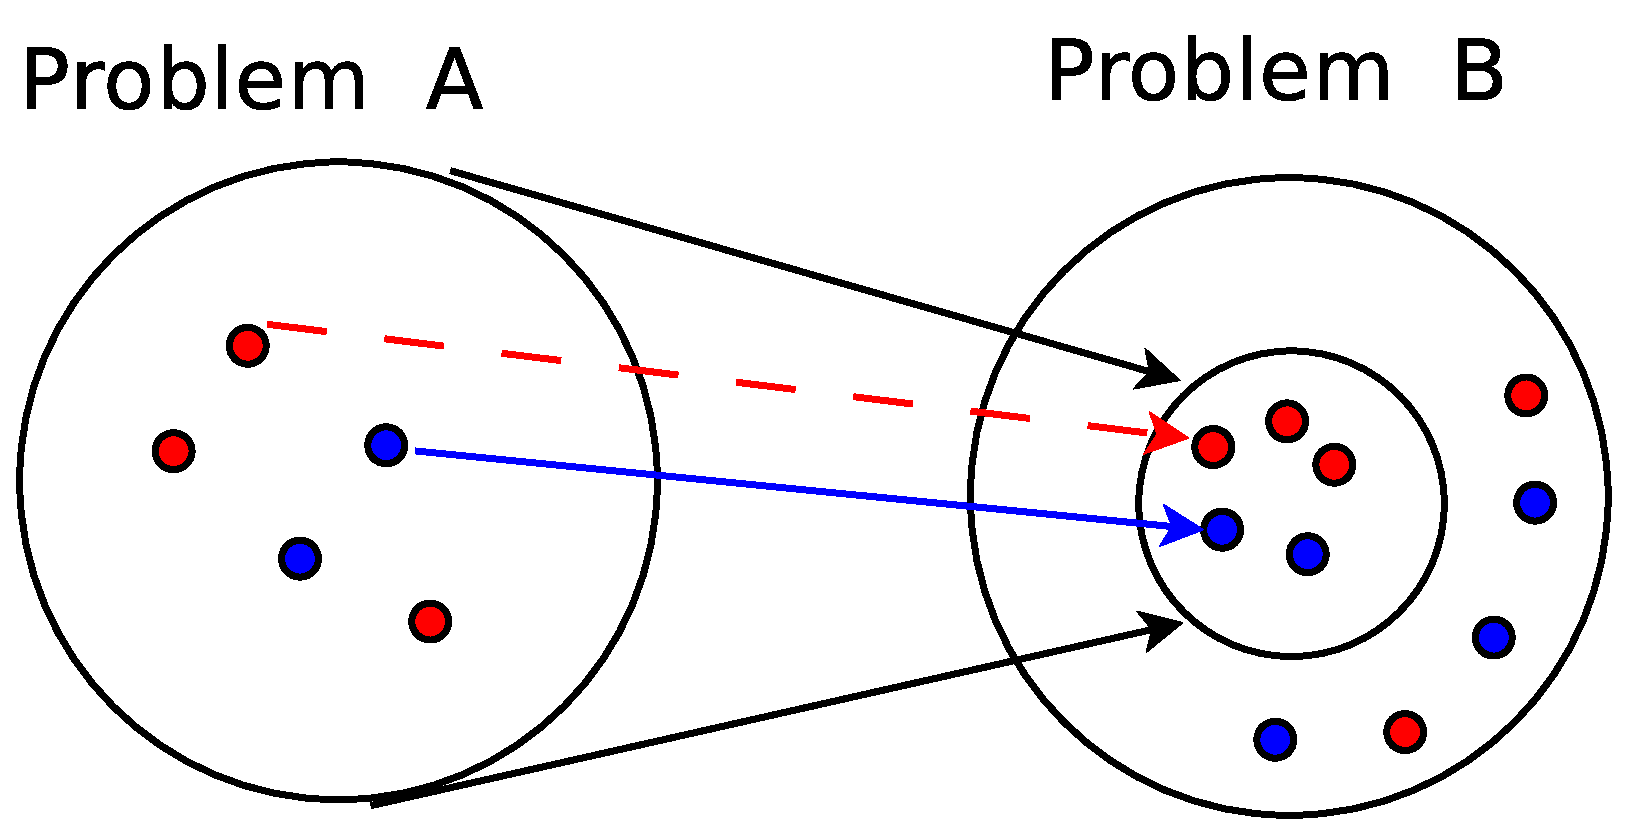
\includegraphics[width=1.5in]{L3-reduction.eps}
\end{figure}
}


\frame{
\frametitle{Recall the NP-Hardness proof of {\sc Independent Set}  }

\begin{itemize}
 \item 
   For a given $SAT$ instance $\phi$ with $k$ clauses, constructing an {\sc Independent Set} instance $(G, k')$ as follows: 
\begin{enumerate}
 \item $G$ consists of $k$ triangles: each triangle corresponds to a clause $C_i$; the nodes are labeled with the literals; connecting $x_i$ and $\neg x_i$ with an edge; \\

 \item Set $k' = k$; 
\end{enumerate}
\item 
Example: 

$ (x_1 \vee x_2 \vee x_3) \wedge ( \neg x_1 \vee x_5 \vee x_6 )$ 


\begin{figure}
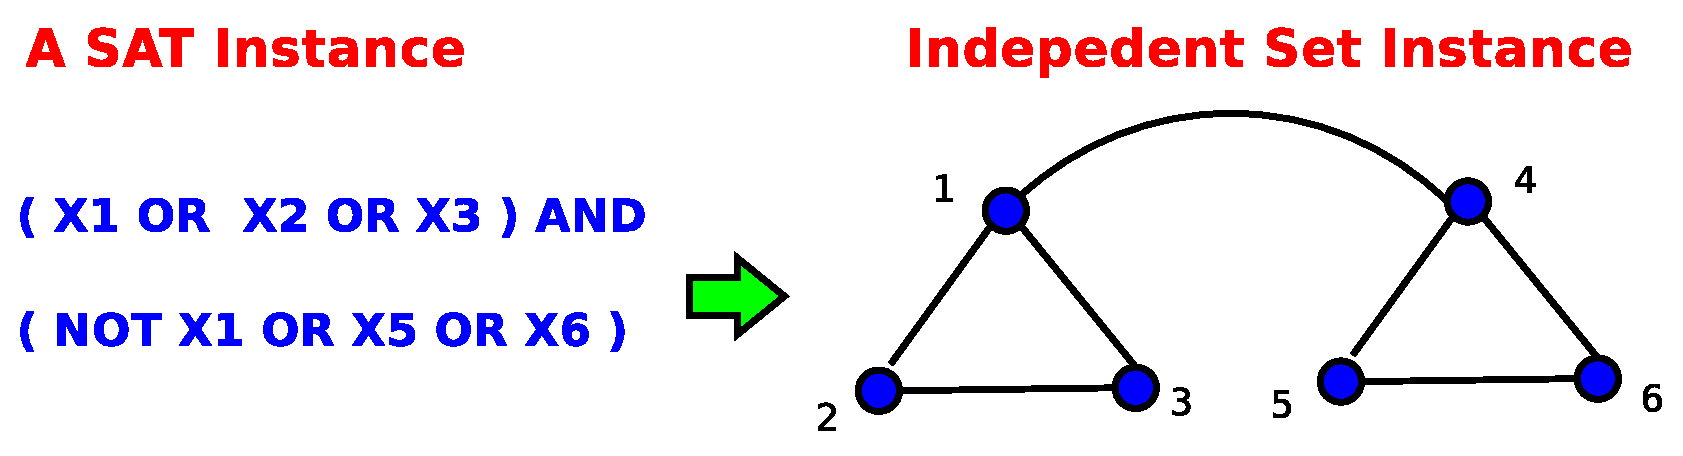
\includegraphics[width=3in]{L3-satindependentset.eps}
\end{figure}

\item 
Intuition: edge represents ``conflicts''; we should identify $k$ nodes (each node from a triangle) without connections (no conflict);
\end{itemize}
}



\frame{
\frametitle{ A way to deal with NP-Hard problems}
\begin{itemize}
 \item NP-Completeness just means that the \textcolor{red}{ the worst-case} instances of the problem are very difficult and unlikely to be solvable in polynomial time. 
\item However, on a \textcolor{red}{particular practial} instance, it is possible that we are not really in the worst case---the instance we're looking at might have some \textcolor{red}{special problem structure} that makes our task easier. 
\item What special problem structure can we utilize? 
\begin{enumerate}
 \item Special parameter: The instance is easier when parameters are small;
 \item Special input structure: The instance is easier if we require the input to be a tree(a special graph); 
 \item Extension: ``tree-like'' graph, a special class of graph with small {\it tree-width}; 
\end{enumerate}
\end{itemize}
}

\frame{
\begin{block}{}
Sovling NP-Hard problems when parameters are small: the iteration number is limited
\end{block}
}


\frame{
\frametitle{ Small parameter:  Parameterized complexity and FPT problems }

\begin{itemize}
 \item 
In computer science, parameterized complexity (also called Fixed-Parameter Tractability) is a measure of complexity for problems with multiple input parameters [R. Downey, M Fellows, 99]. 
\item 
Motivation: Some hard problems can be solved by algorithms that are exponential only in the size of a fixed parameter $k$ while polynomial in the size of the input size $n$, say, $T(n,k) = O( 2^k ploy(n))$.
% Such an algorithm is called a fixed-parameter tractable (FPT)algorithm, because the problem can be solved efficiently for small values of the fixed parameter. 
\item Hence, if $k$ is fixed at a small value, such problems can still be considered 'tractable' despite their traditional classification as 'intractable'.

\end{itemize}
} 

\frame{ 
\frametitle{ Two examples } 


\begin{enumerate}
\item 
For the {\sc VertexCover} problem, the parameter can be the number of vertices in the cover. 
\item When modeling error correction, one can assume the error (denoted as $k$) to be "small" compared to the total input size. Then it is interesting to see whether we can find an algorithm which is exponential only in $k$, and not in the input size.
\end{enumerate}
}


\frame{
\frametitle{ Example: finding small vertex covers }

Intuition: Given a graph $G=<V,E>$, how many guards should be deployed on nodes to surveille ALL the paths?

\begin{block}{Formalized Definition:}
 {\bf Input:} Given a graph $G=<V,E>$, and an integer $k$, \\
 {\bf Output:} is there a set of nodes $S\subseteq V$, $|S| \le k$, such that each edge has at least one of its endpoints in $S$? 
\end{block}

\begin{figure}
        \centering
        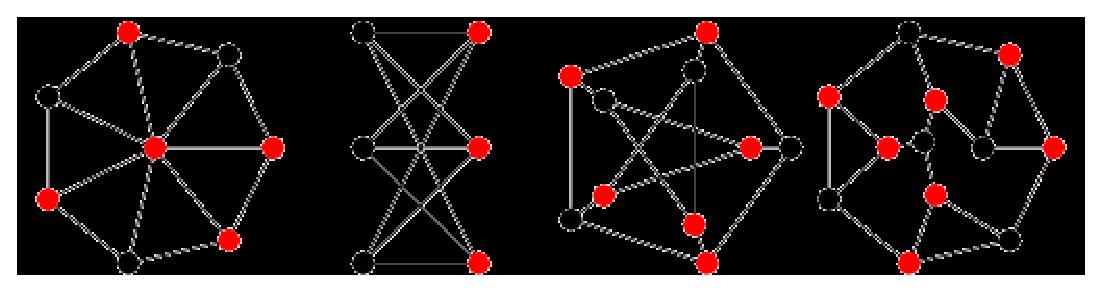
\includegraphics[width=2.8in]{L3-vertexcover-example.eps}
\end{figure}
}

\frame{
\frametitle{ Trial 1: a brute-force algorithm } 

\begin{itemize}
 \item Brute-force algorithm: enumerating all possible subsets of $V$ of size $k$. 
 \item Time-complexity: $O( k n { {n}\choose{k} } ) = O(k n^{k+1})$. (There are  ${ {n}\choose{k} }$ subsets, and it takes $O(kn)$ time to check whether a subset is a vertex cover.)
 \item Note: The brute-force algorithm is a polynomial time algorithm when $k$ is a fixed constant (e.g., $k=2$ or $k=3$). %In other words, the intractability sets in for real once $k$ grows as a function of $n$. 
\end{itemize}
}

\frame{
\frametitle{ Trial 1: a brute-force algorithm  cont'd} 
\begin{itemize}
 \item However, even for moderately small values of $k$, (say $n=1000$ and $k=10$), a running time of $O(kn^{k+1})$ is quite impractical.
 \item In contrast, an algorithm with the running-time of $O(k2^k n)$ is appealing since:
\begin{enumerate}
 \item The algorithm will be practical even when $n=1000$ and $k=10$; 
 \item The expoential dependence on $k$ has been moved out of the exponent on $n$ and into a separate function. 
\end{enumerate}
 \item Question: can we break out the interaction of $n$ and $k$? 
\end{itemize}
} 


\frame{
\frametitle{Trial 2: Limited enumeration }
\begin{itemize}
\item 
Basic idea: Perform limited enumeration. Enumerate all $2^k$ possibilities for $k$ arbitrarily chosen edges; 
\begin{enumerate} 
  \item Consider any edge $e=(u,v)$. In $any$ $k$-node vertex cover of $G$, either $u$ or $v$ should belong to vertex cover $S$. 
 \item Suppose that $u$ belongs to $S$. Then if we delete node $u$ and all incident edges, we obtain a new graph $G-\{u\}$, and there should be a vertex cover of $G'=G-\{u\}$ of size at most $k-1$. 
\end{enumerate}
\end{itemize} 

\begin{figure}
        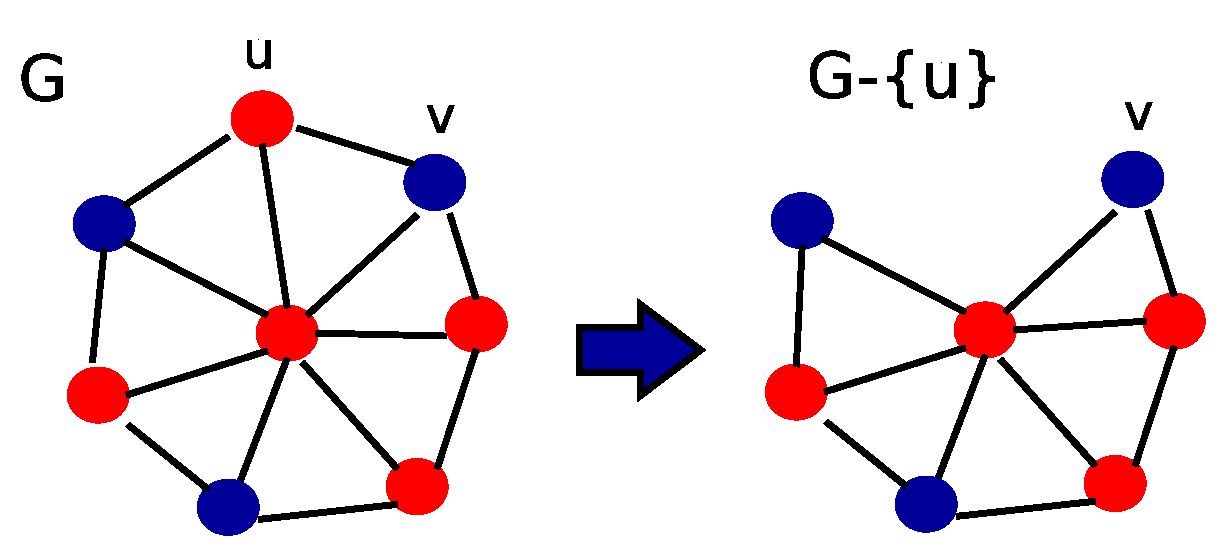
\includegraphics[width=2.0in]{L13-vertexcoverg-u.eps}
\end{figure}
} 


\frame{
\frametitle{Limited enumeration: correctness }

\begin{Theorem}
 Let $e=(u,v)$ be any edge of $G$. $G$ has a vertex cover of size at most $k$ iff $G-\{u\}$ or $G-\{v\}$ has a vertex cover of size at most $k-1$. 
\end{Theorem}
\begin{Proof}
\begin{itemize}
\item 
$\Leftarrow$ \\ Obvious. \\
\item 
$\Rightarrow$ \\ 
	\begin{itemize}
		\item 
	Suppose $S$ is a vertex cover with size at most $k$, and $u\in S$. 
	\item Then $S-\{u\}$ must cover all edges except the edges incident  to $u$. 
	\end{itemize}
\end{itemize}
\end{Proof}
} 

\frame{
\begin{small}
Algorithm $VertexCover( G, k )$
\begin{algorithmic}[1]
\IF {$G = \{\} $} 
\RETURN  $\{\}$; 
\ENDIF; 
\IF { $| G | > k | V | $ } 
\RETURN ``Infeasible'';
\ENDIF
\STATE \textcolor{red}{Arbitrarily} select an edge $e=<u,v>$; 
\STATE $S_u = VertexCover( G-\{u\}, k-1 )$; 
\STATE $S_v = VertexCover( G-\{v\}, k-1 )$; 
\IF { $S_u \neq Infeasible $}
\RETURN $S_u \cup \{u\}$; 
\ELSIF{ $S_v \neq Infeasible $}
\RETURN $S_v \cup \{v\}$; 
\ELSE 
\RETURN Infeasible; 
\ENDIF
\end{algorithmic}
\end{small}
Note: If $G=(V,E)$ has $n$ nodes and a vertex cover $S$ of size $k$, then $G$ has at most $k(n-1)$ edges. (Reason: each node in $S$ covers at most $n-1$ edges since the maximum degree is $n-1$.)
}

\frame{
\frametitle{Analysis}

\begin{figure}
        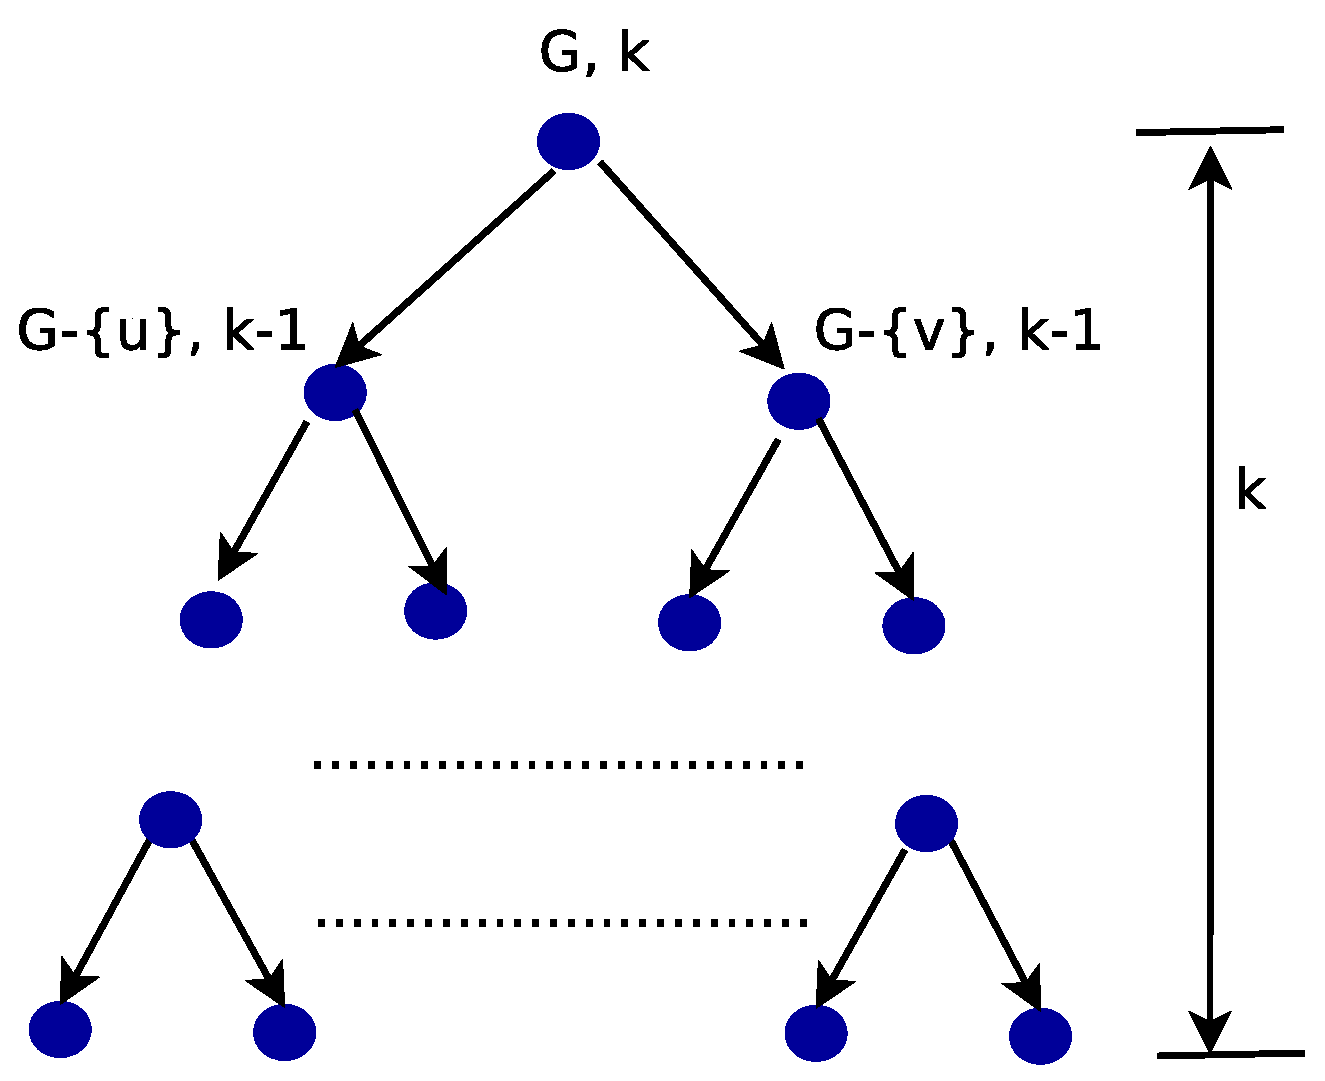
\includegraphics[width=2in]{L13-vertexcoveralgorithmanalysis.eps}
\end{figure}
\begin{Theorem}
 The recursive algorithm cost $O(k 2^k n)$ time.
\end{Theorem}
} 

\frame{
\frametitle{Analysis: Induction proof }
\begin{Proof}
\begin{itemize}
\item 
 Let $T(n,k)$ be the running time of searching a vertex cover with size of $k$ on a graph with $n$ nodes. 
 \item We have: 
\begin{eqnarray} 
 T(n,1) &\leq& cn \\
 T(n,k) &\leq& 2 T(n-1,k-1) + c k n   
\end{eqnarray}
\item  Suppose $T(n,k-1) \leq c k 2^{k} n$. Then we have: 
\begin{eqnarray} 
 T(n,k) &\leq& 2 T(n-1,k-1) + c k n \\   
&\leq& 2 c (k-1) 2^{k-1} n + c k n \\ 
&=& c (k-1) 2^k n + c k n \\
&\leq& c k 2^k n
\end{eqnarray}
\end{itemize}
\end{Proof}
}

\frame{
\begin{block}{}
 Solving NP-Hard problems on trees: no communications among sub-problems
\end{block}
}


\frame{
\frametitle{Solving NP-Hard problem on trees}
\begin{itemize}
 \item Another favor of specical structure: not when the natural ``size'' parameters are small, but when the problem structure is ``simple'';
 \item Tree is a simple graph: on a tree, a problem can be decomposed into ``independent''  sub-problems. Thus, the communication between sub-problems are broken. 
 \item In fact, it has been found that many NP-Hard graph problems can be solved efficiently when the underlying graph is tree. 
 \end{itemize}
\begin{figure}
        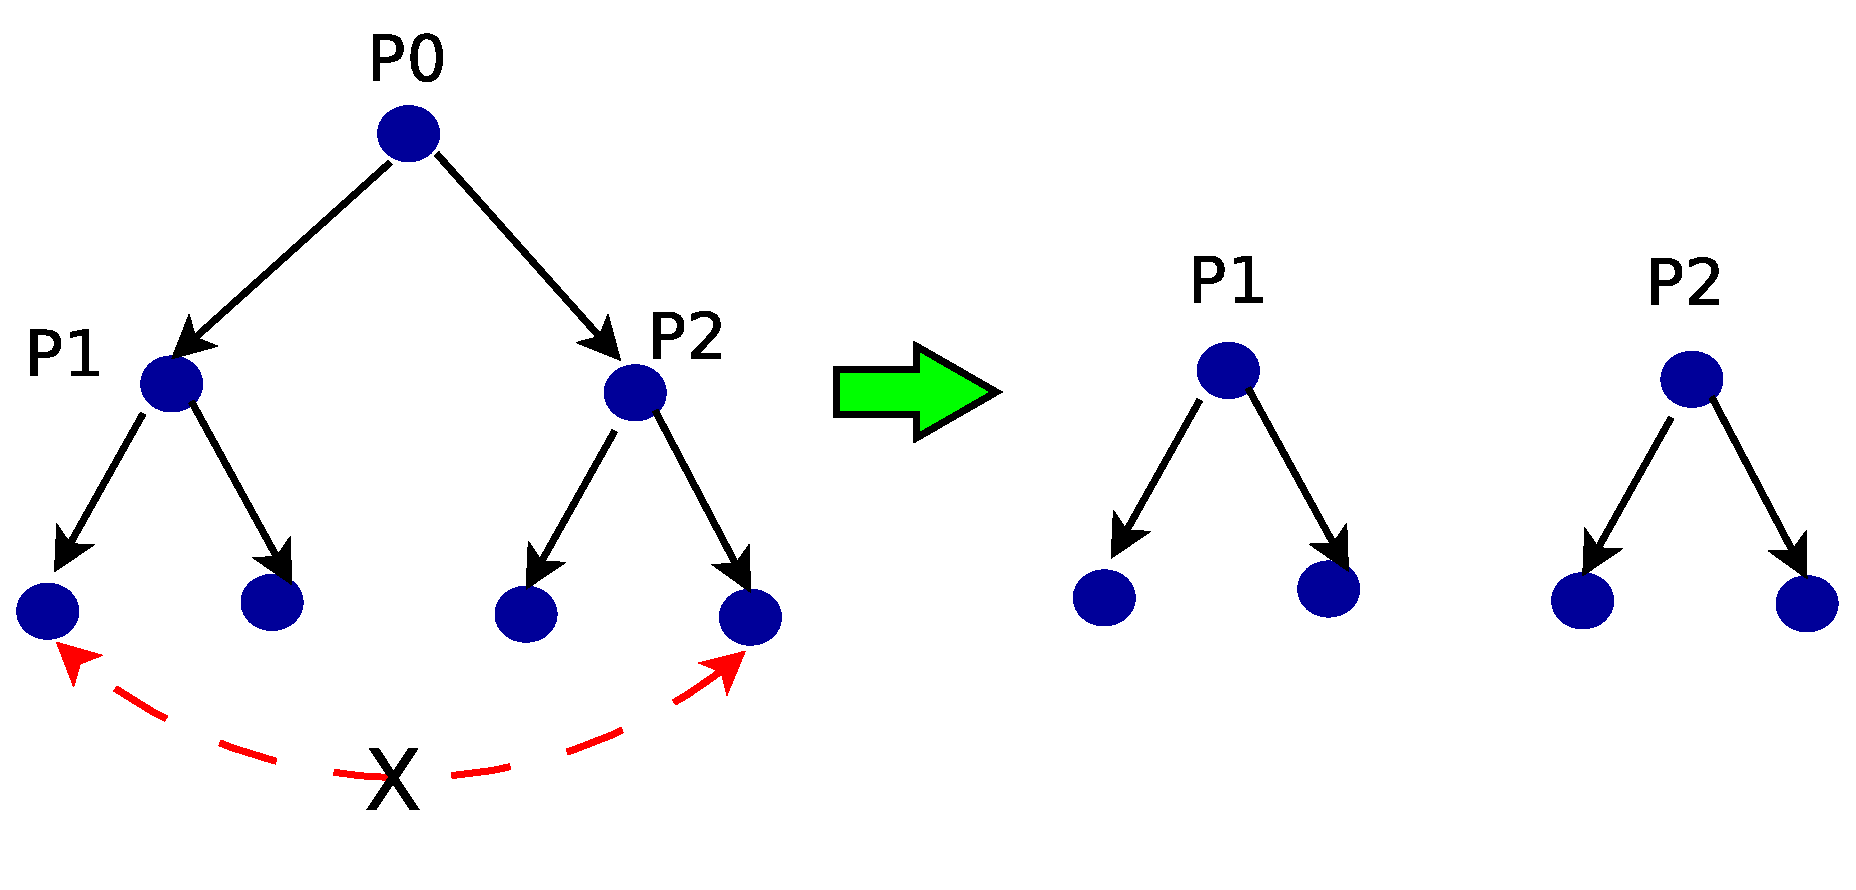
\includegraphics[width=3in]{L13-solvingNPHardproblems.eps}
\end{figure}
}

\frame{
\frametitle{ An example: {\sc Independent Set} Problem}
Practical Problem: \\
 	Suppose you have $n$ friends, and some pairs of them don't get along. How to invite at least $k$ of them to dinner if you don't want any interpersonal tension? 

\begin{block}{Formalized Definition:}
 {\bf Input:} Given a graph $G=<V,E>$. Each node $u\in V$ has a weight $w(u) \geq 0 $.   \\
 {\bf Output:} to find a set of nodes $S\subseteq V$  such that no two nodes in $S$ are joined by an edge and $\sum_{v \in S} w(v)$ is maximized. 
\end{block}
\begin{figure}
        \centering
        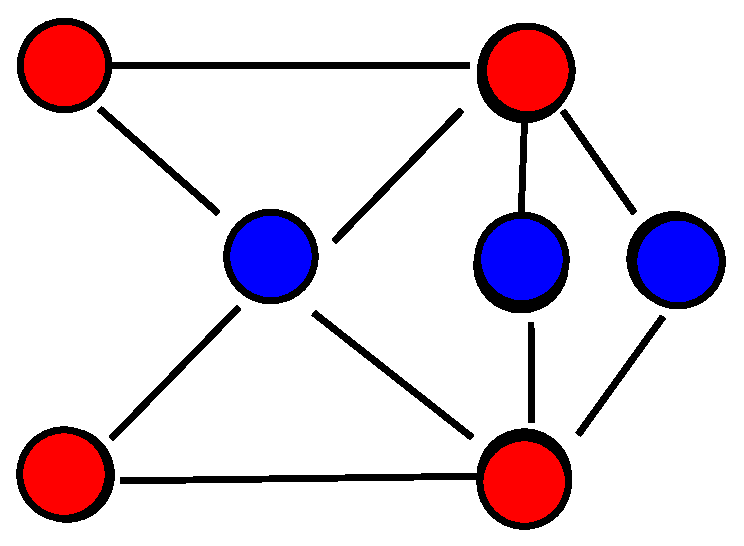
\includegraphics[width=1.0in]{L3-independentset.eps}
\end{figure}
}
% 
% \frame{
% \frametitle{ {\sc Independent Set} -- another intersting instance}
% \begin{figure}
%  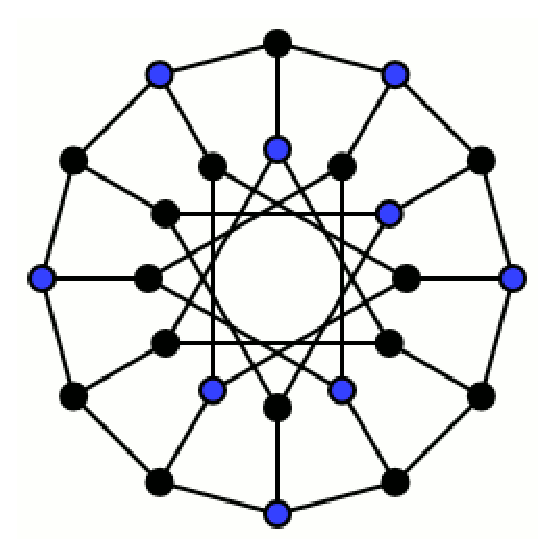
\includegraphics[width=1.5in] {Independent_set_graph.eps}
% \end{figure}
% The set of 9 blue vertices is an independent set for this graph of 24 vertices.
% }

\frame{
\frametitle{Recall the  NP-Hardness proof of {\sc Independent Set} problem}

\begin{figure}
 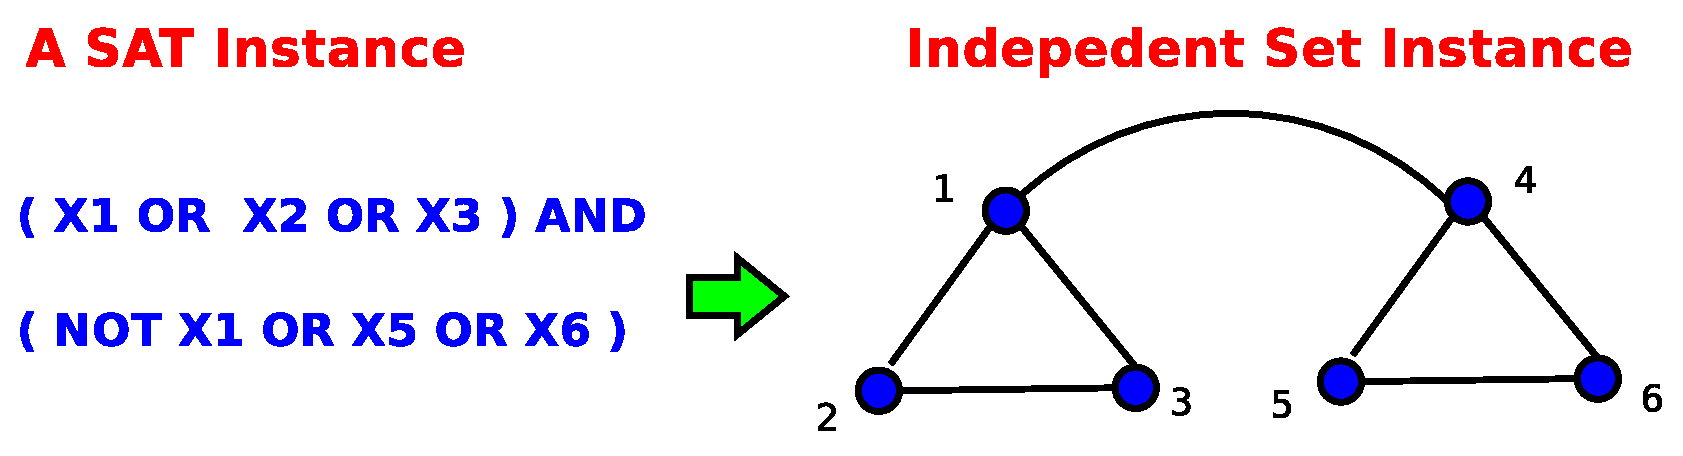
\includegraphics[width=3.5in]{L3-satindependentset.eps}
\end{figure}

\begin{itemize}
	\item Note: the generated graph is very special
	\item Question: is the problem still hard when the underlying graph is a tree? 
\end{itemize} 
}


\frame{
\frametitle{ {\sc Independent Set} problem is easy when $G$ is a tree. }

\begin{enumerate}
\item Solution: a set of nodes. Imagine the solving process as a series of \textcolor{red}{decisions}; each decision is to select a node. 
\item Suppose we have already worked out the optimal solution $O$, where the first \textcolor{red}{decision} is made for root node $u$. There are a total of $2$ options for this step: 
\begin{enumerate}
\item Select $u$: This decision decomposes the original problem into several  \textcolor{red}{independent} sub-problems, i.e., solving smaller sub-problems for each sub-trees. 
\item  Do not select $u$: This decision also decomposes the original problem into several  \textcolor{red}{independent} sub-problems. 
\end{enumerate}
\item Thus, we can design the general form of sub-problems as: selecting independent nodes when the root is seleted or not selected. 
\end{enumerate}
} 

\frame{
\frametitle{ {\sc Independent Set} problem is easy when $G$ is a tree }

 
\begin{figure}
 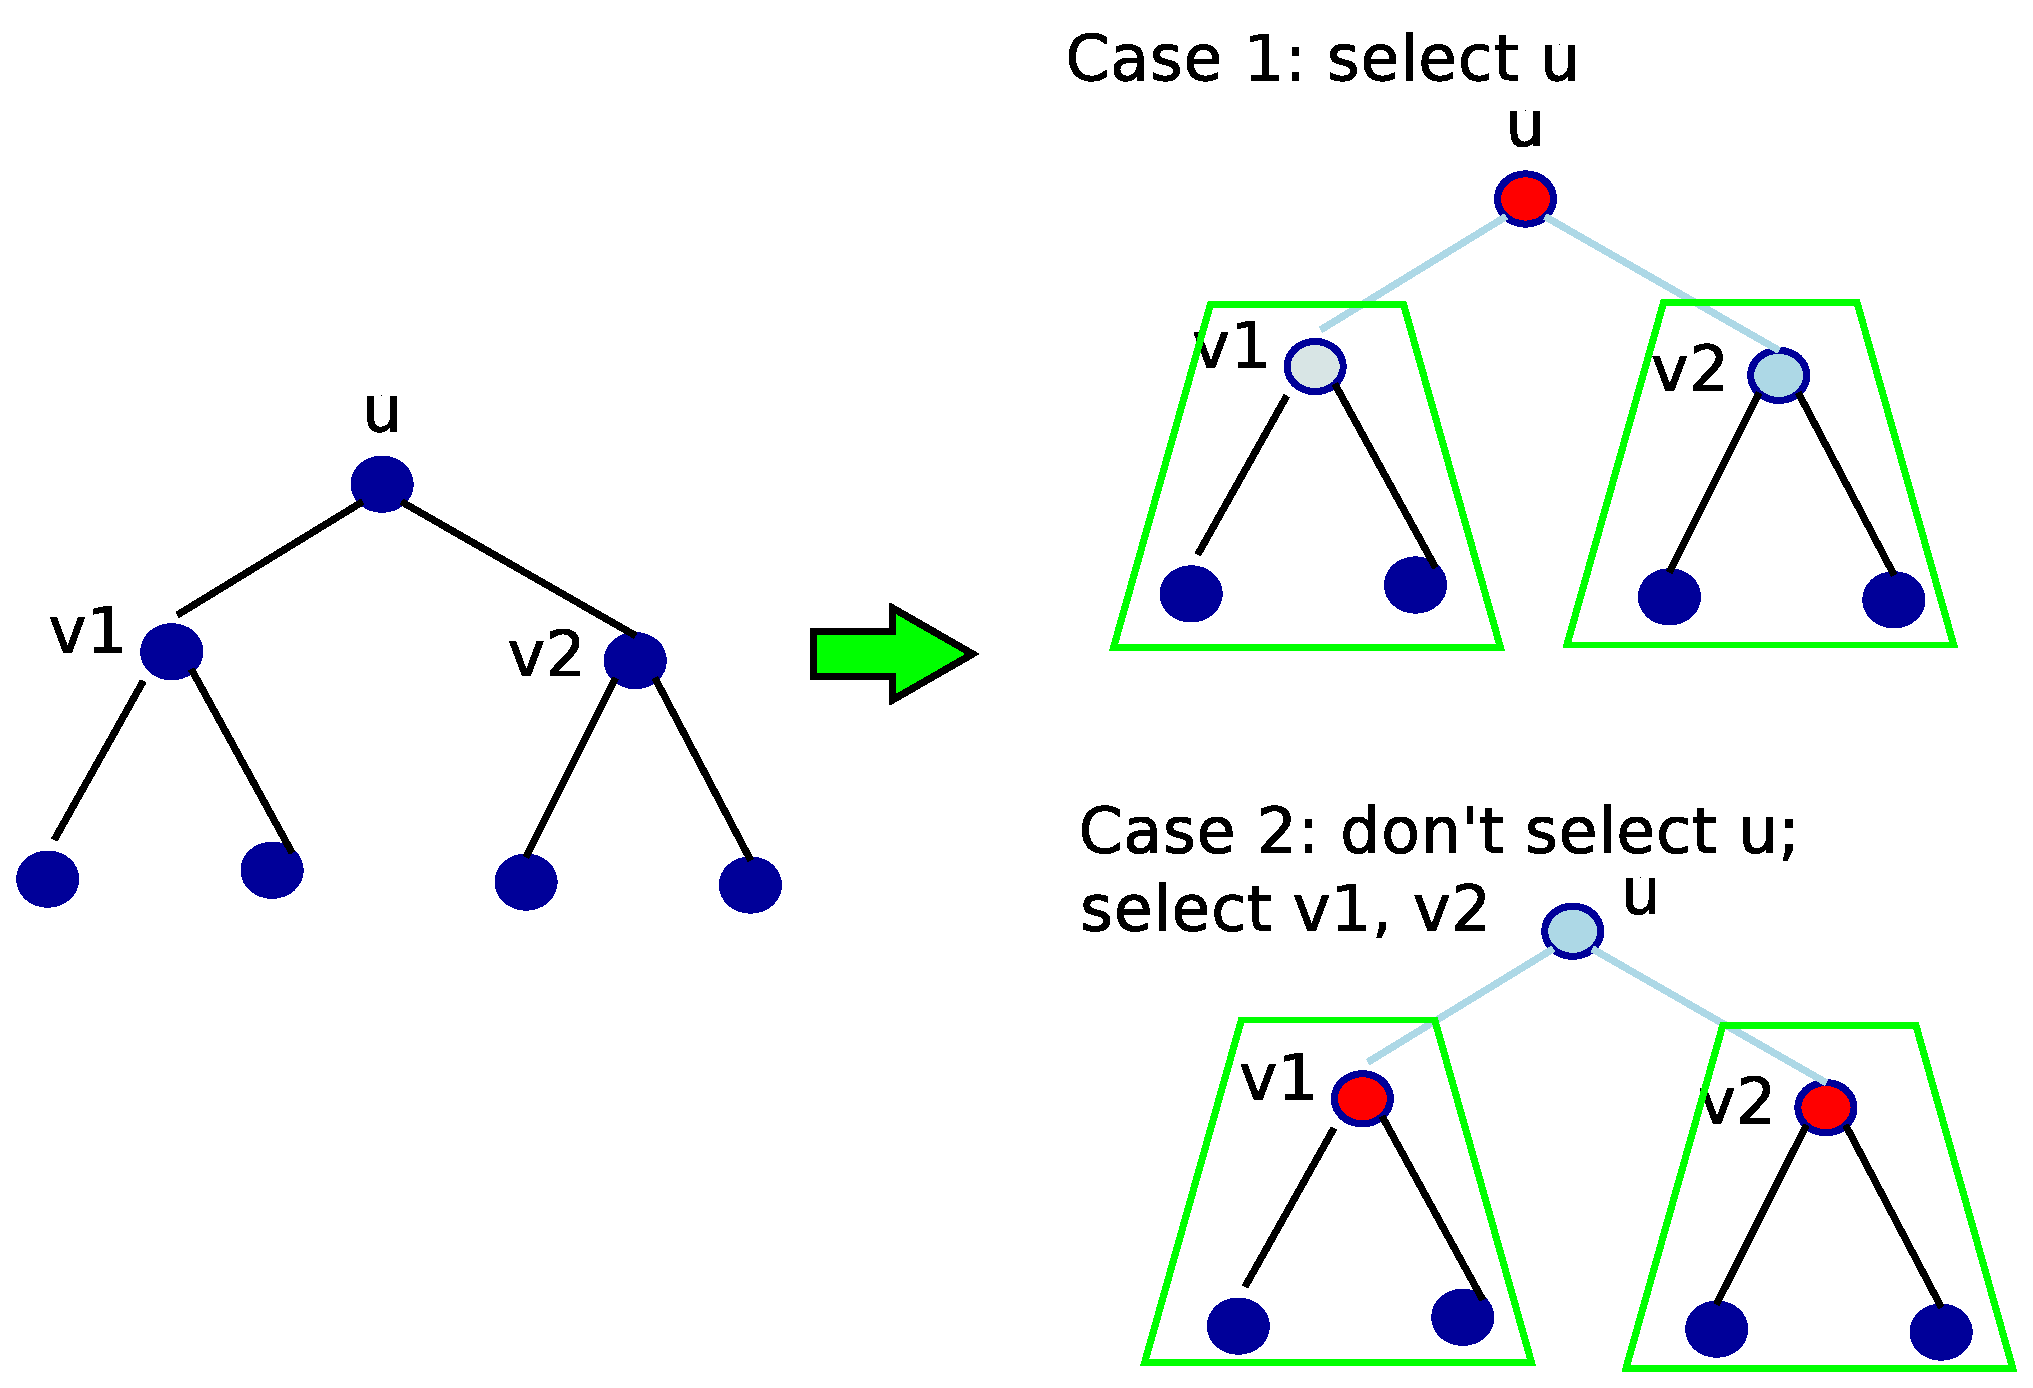
\includegraphics[width=3in] {L13-independentsetalgorithmexample.eps}
\end{figure}
} 

\frame{
\frametitle{ A dynamic programming algorithm } 
\begin{small} 
\begin{itemize}
\item General form of sub-problems: to find the maximum weighted independent set $S(u)$ in sub-tree $T(u)$. Here, $T(u)$ refers to the sub-tree with node $u$ as its root.  
\item There are only two cases: $u\in S(u)$, and $u\notin S(u)$. In the case $u\notin S(u)$, we can include all children of $u$ in $S(u)$. 
\item Optimal substructure: Let $OPT_{in}(u)$ be the maximum weight when $u\in S(u)$, and $OPT_{out}(u)$ be the maximum weight when $u\notin S(u)$. We have the following recursions:
\begin{eqnarray}
OPT_{in}(u) &=& w_u + \sum_{\text{v is a child of u} } OPT_{out}(v) \\
OPT_{out}(u) &=& \sum_{\text{v is a child of u} } \max\{OPT_{out}(v),OPT_{in}(v)\} 
\end{eqnarray}
and
\begin{eqnarray}
OPT_{in}(u) &=& w_u  \text{\qquad if $T(u)=\{\}$}  \\
OPT_{out}(u) &=& 0 \text{\qquad\quad if $T(u)=\{\}$}
\end{eqnarray}
\end{itemize}
\end{small}
} 


\frame{ 
\frametitle{ Dynamic programming algorithm } 
$MaximumIndependentSetDP(  T )$
\begin{algorithmic}{}
\FOR { all nodes in $T$ in posterior order } 
\IF { $u$ is a leaf } 
\STATE $M_{out}[u] = 0;$; 
\STATE $M_{in}[u] = w(u);$;
\ELSE
\STATE $M_{out}[u] = \sum_{ v \in son(u)} \max \{M_{out}[v], M_{in}[v] \};$; 
\STATE $M_{in}[u] = w_u + \sum_{ v \in son(u)} M_{out}[v];$;
\ENDIF
\ENDFOR 
\RETURN $\max\{M_{in}[root], M_{out}[root]\};$
\end{algorithmic}

Time-complexity: $O(n)$. (Reason: we calculate $M_{in}$ and $M_{out}$ in a bottom-up manner; at each node $u$, only $O(d)$ time is needed, where $d$ denotes the number of children of $u$.) 
}

\frame{
\frametitle{ From DP to Greedy when $w(u)=1, \forall u \in V$. }
\begin{itemize} 
%  \item Key observation: problem can be decomposed into sub-problems. 
 \item Greedy selection: Consider an edge $e=(u,v)$, where $v$ is a leaf. Then there exists a maximum independent set containing   $v$ (Why? exchange argument).  
 \end{itemize}
\begin{figure}
 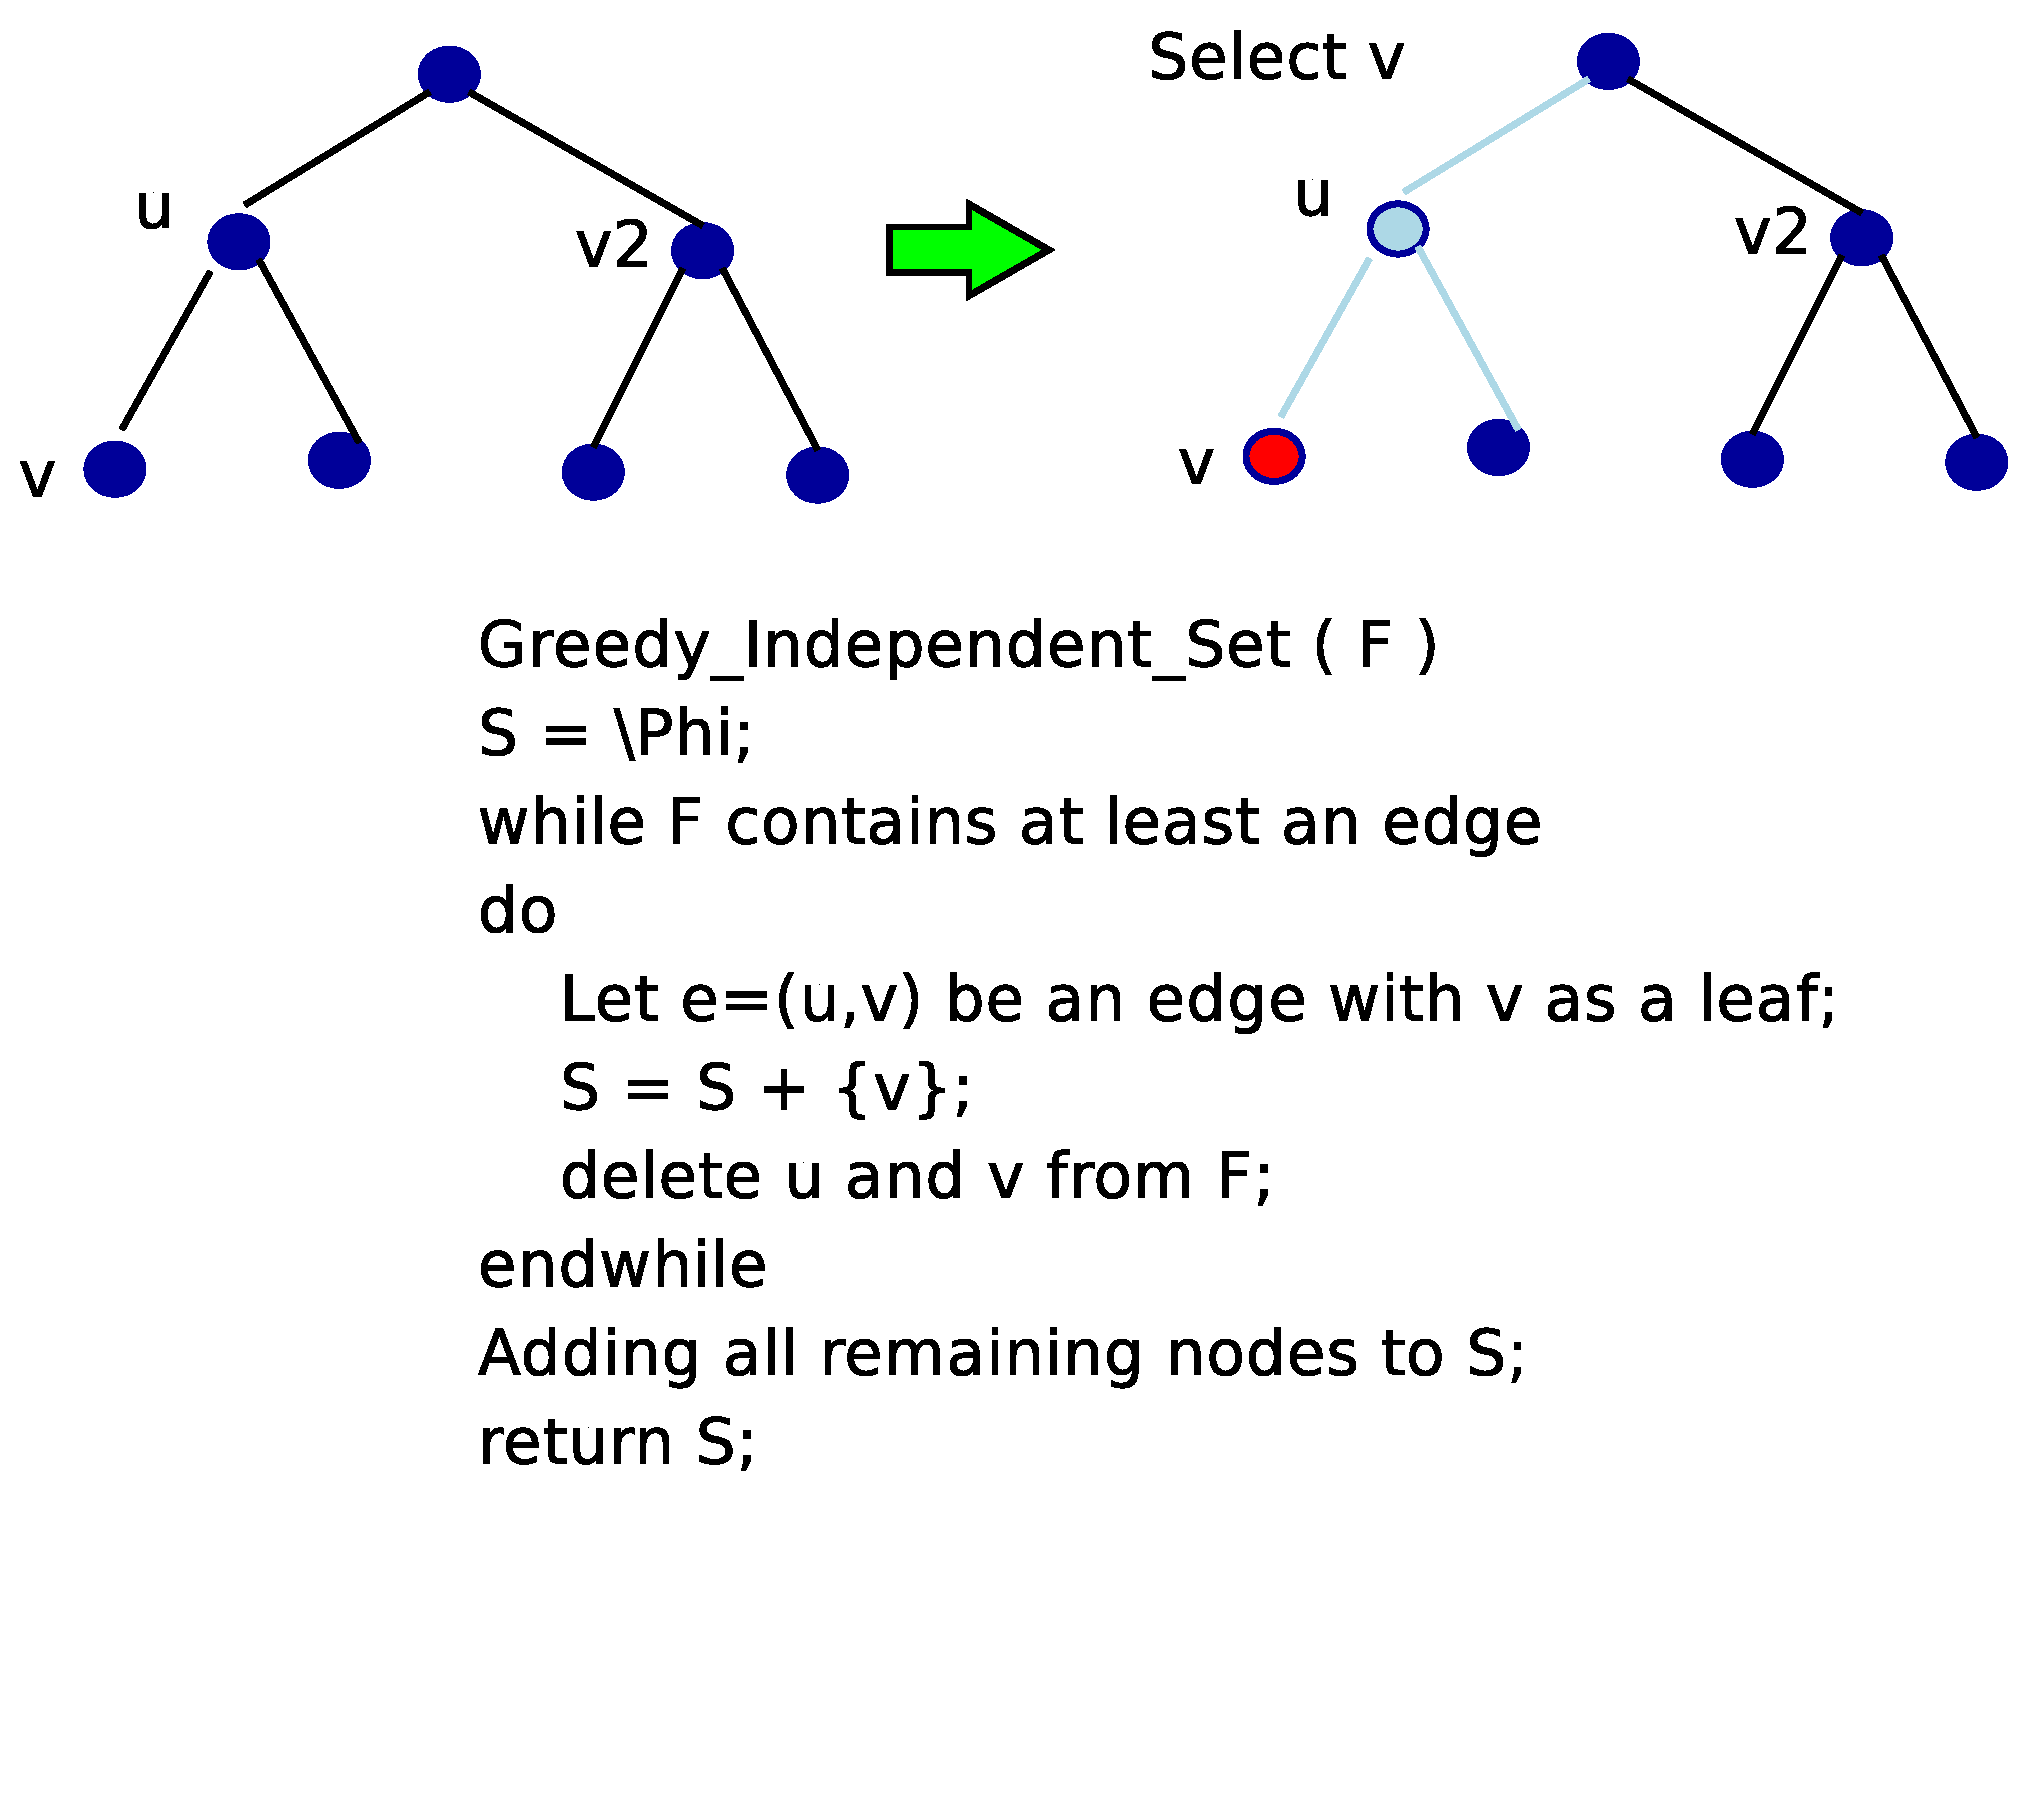
\includegraphics[width=2.5in] {L13-independentsetgreedyalgorithmexample.eps}
\end{figure}

\begin{itemize}
\item 
Note: removing node $u$ may change a tree to a forest. 
\item 
Time-complexity: $O(n)$ again. 
\end{itemize}
}

\frame{
\begin{block}{}
 Solving NP-Hard problem on tree-like graph: the connection among sub-problems is small
\end{block}
} 

\frame{
\frametitle{ Extension of tree: ``tree-like'' graph } 

\begin{itemize}
 \item Why the {\sc IndependentSet} problem becomes tractable when the underlying graph is a tree? 
 \item Reason: the communication between sub-problems is broken by removing ONE node, i.e., the sub-problem are independent. 
 \item A weak question: If the removal of ONE node cannot completely cut all communication between sub-problems, can we achieve this goal through removing a SMALL SET of nodes? 
 \end{itemize}
 } 
 
\frame{
\frametitle{ Tree-like graph } 
\begin{figure}
 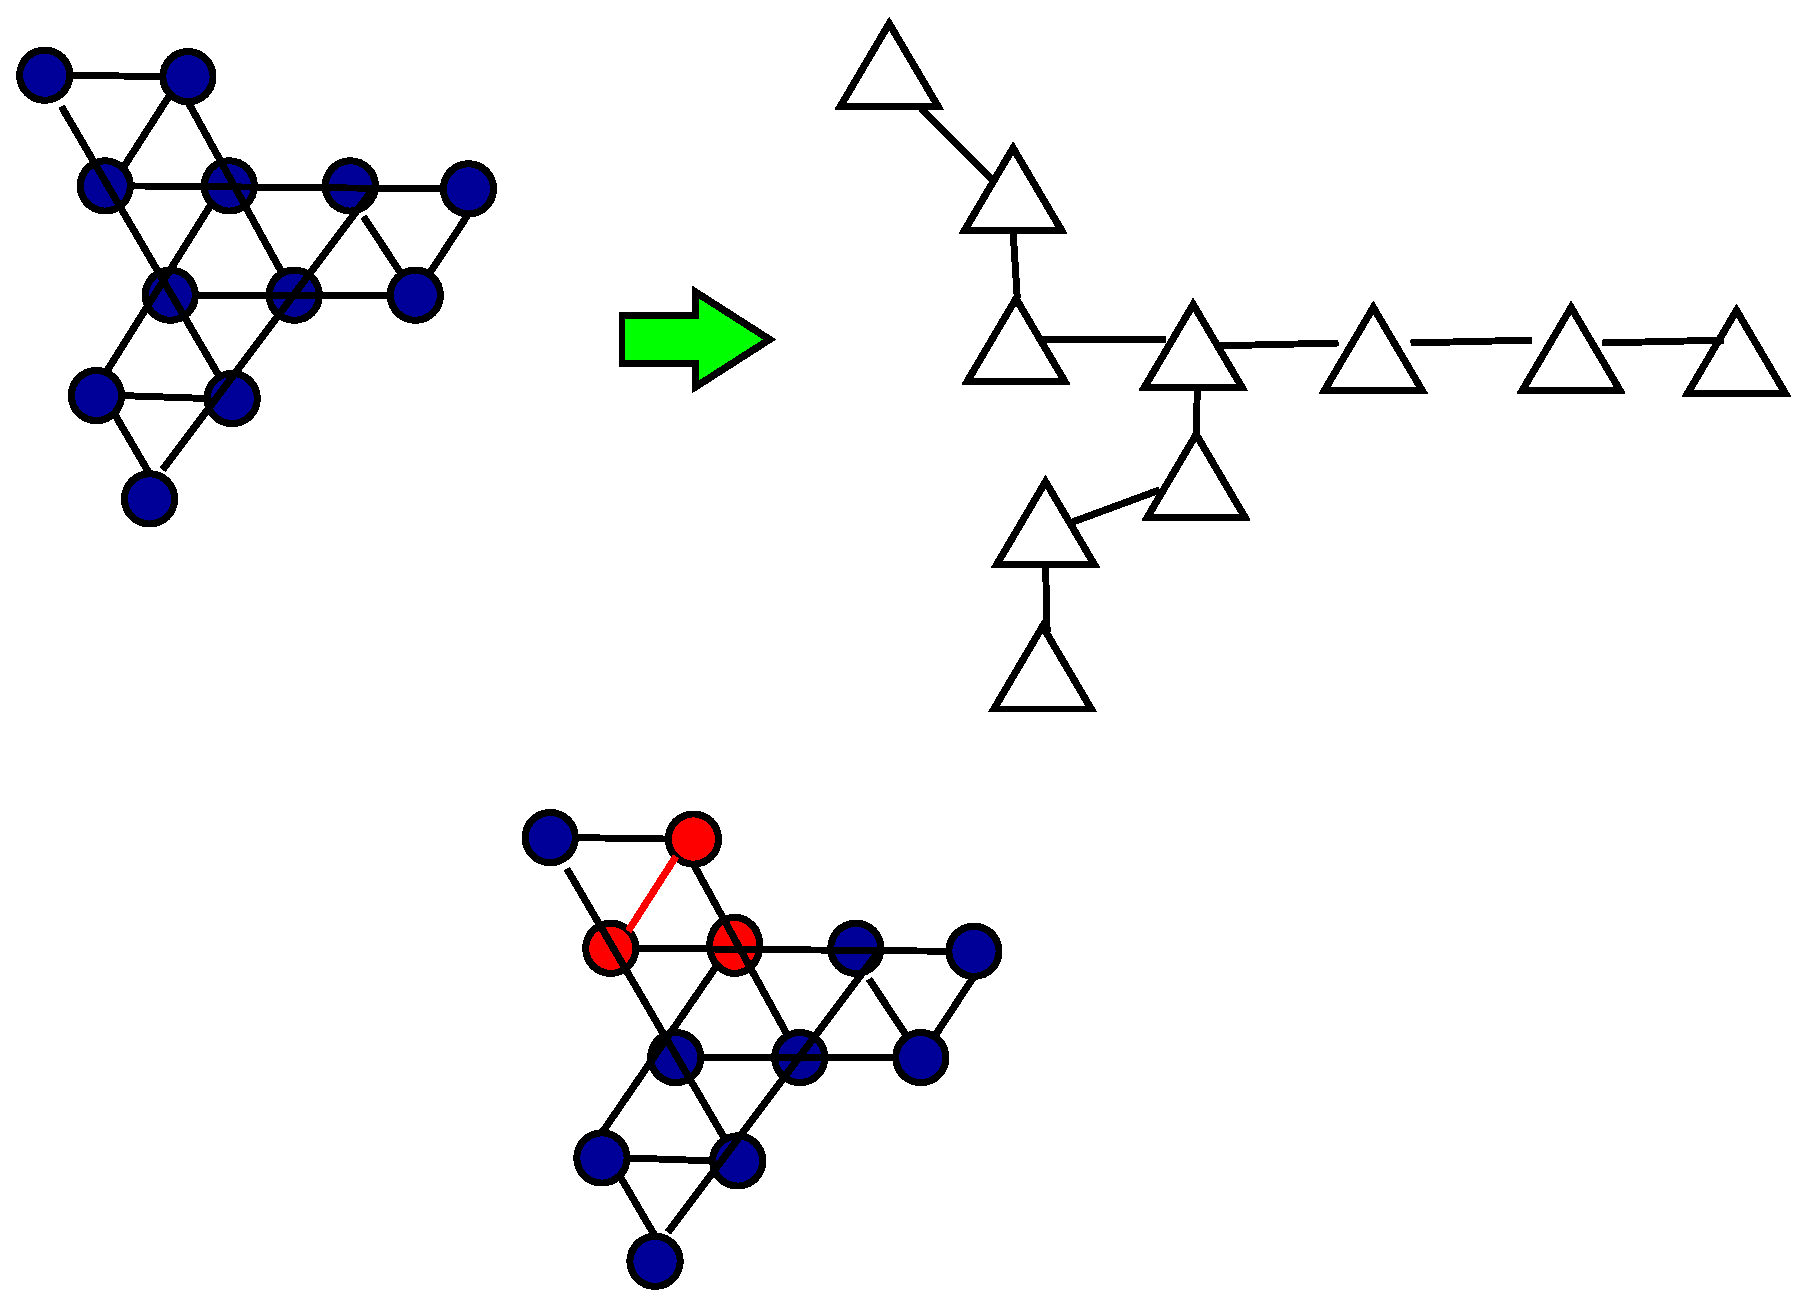
\includegraphics[width=2.5in] {L13-treelikegraph.eps}
\end{figure}
\begin{itemize}
\item Observations: 
\begin{enumerate}
 \item There might be  many cycles in NODE level; however, it is a tree in TRI-ANGLE level. 
 \item Removal of a NODE cannot generate independent sub-problems; however, removal of a TRI-ANGLE will decompose the graph into parts. 
\end{enumerate}
\end{itemize}
}

\frame{
\frametitle{How to change a graph into tree? Tree-decomposition}
\begin{definition}[Tree decomposition] 
\begin{itemize}
\item 
A tree-decomposition of a graph $G=(V,E)$ is a tree $T$, where each node $t$ of $T$ corresponds to a subset $V_t \subset V$ (called ``pieces'' of $G$). $T$ and $V_t$ must satisfy the following properties: 
\begin{enumerate}
 \item (Node coverage)  Every node of $G$ belongs to at least one piece $V_t$. 
 \item (Edge coverage)  The two end nodes of an edge should be covered by a piece $V_t$.
 \item (Coherence) In tree $T$, if $t_2$ is in a path from $t_1$ to $t_3$, then $V_{t_1} \cap V_{t_3} \subseteq V_{t_2}$. 
\end{enumerate}
\end{itemize} 
\end{definition}
} 

%\frame{
%\frametitle{Tree-decomposition: intuition }
%\begin{itemize} 
%\item 
%Define a collection of subsets $V_t \subset V$. 
%\item 
%If two subsets $V_i$ and $V_j$ share common nodes of $G$, then draw an edge to connect $V_i$ and $V_j$. 
%\item Meanwhile, we should  guarantee that there is no cycle among $V_t, t\in T$. 
%\end{itemize} 
%\begin{figure}
% 	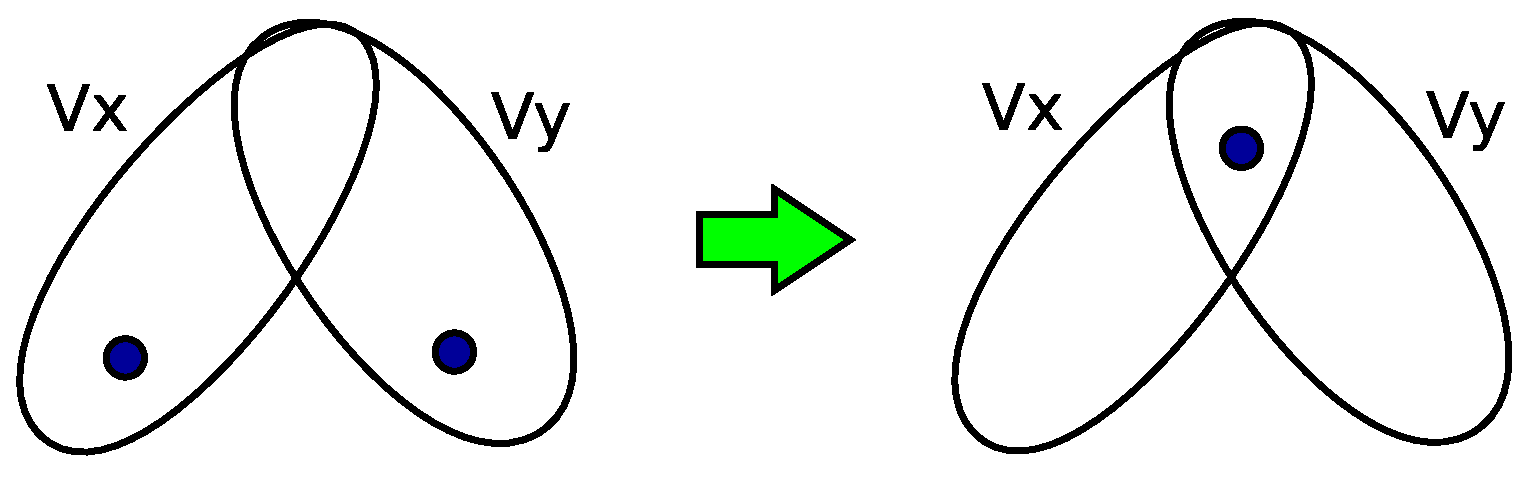
\includegraphics[width=3.5in] {L13-treedecompositioncoherence.eps}
%\end{figure}
%}

\frame{
\frametitle{Properties of tree-decomposition}
\begin{itemize}
\item The important property of tree that makes things easier: 
\begin{enumerate}
 \item Removal an edge: usually decompose the tree into two INDEPENDENT parts; 
 \item Removal a node: usally decompose the tree into a forest containing INDEPENDENT trees; 
\end{enumerate}
\item The coherence property ensure these two properties for the tree-decomposition $T$ of a graph $G$. 
\end{itemize}
} 


\frame{
\frametitle{Removing a node: generating independent sub-problems }

\begin{Theorem} 
(Removing a node) Suppose $T-t$ (a forest) consists of trees $T_1,T_2,...,T_d$. Then the subgraph $G_{T_1} - V_t$, $G_{T_2} - V_t$, ..., $G_{T_d} - V_t$ share no common nodes, and there is no edge connecting any two subgraphs. 
\end{Theorem}
\begin{figure}
 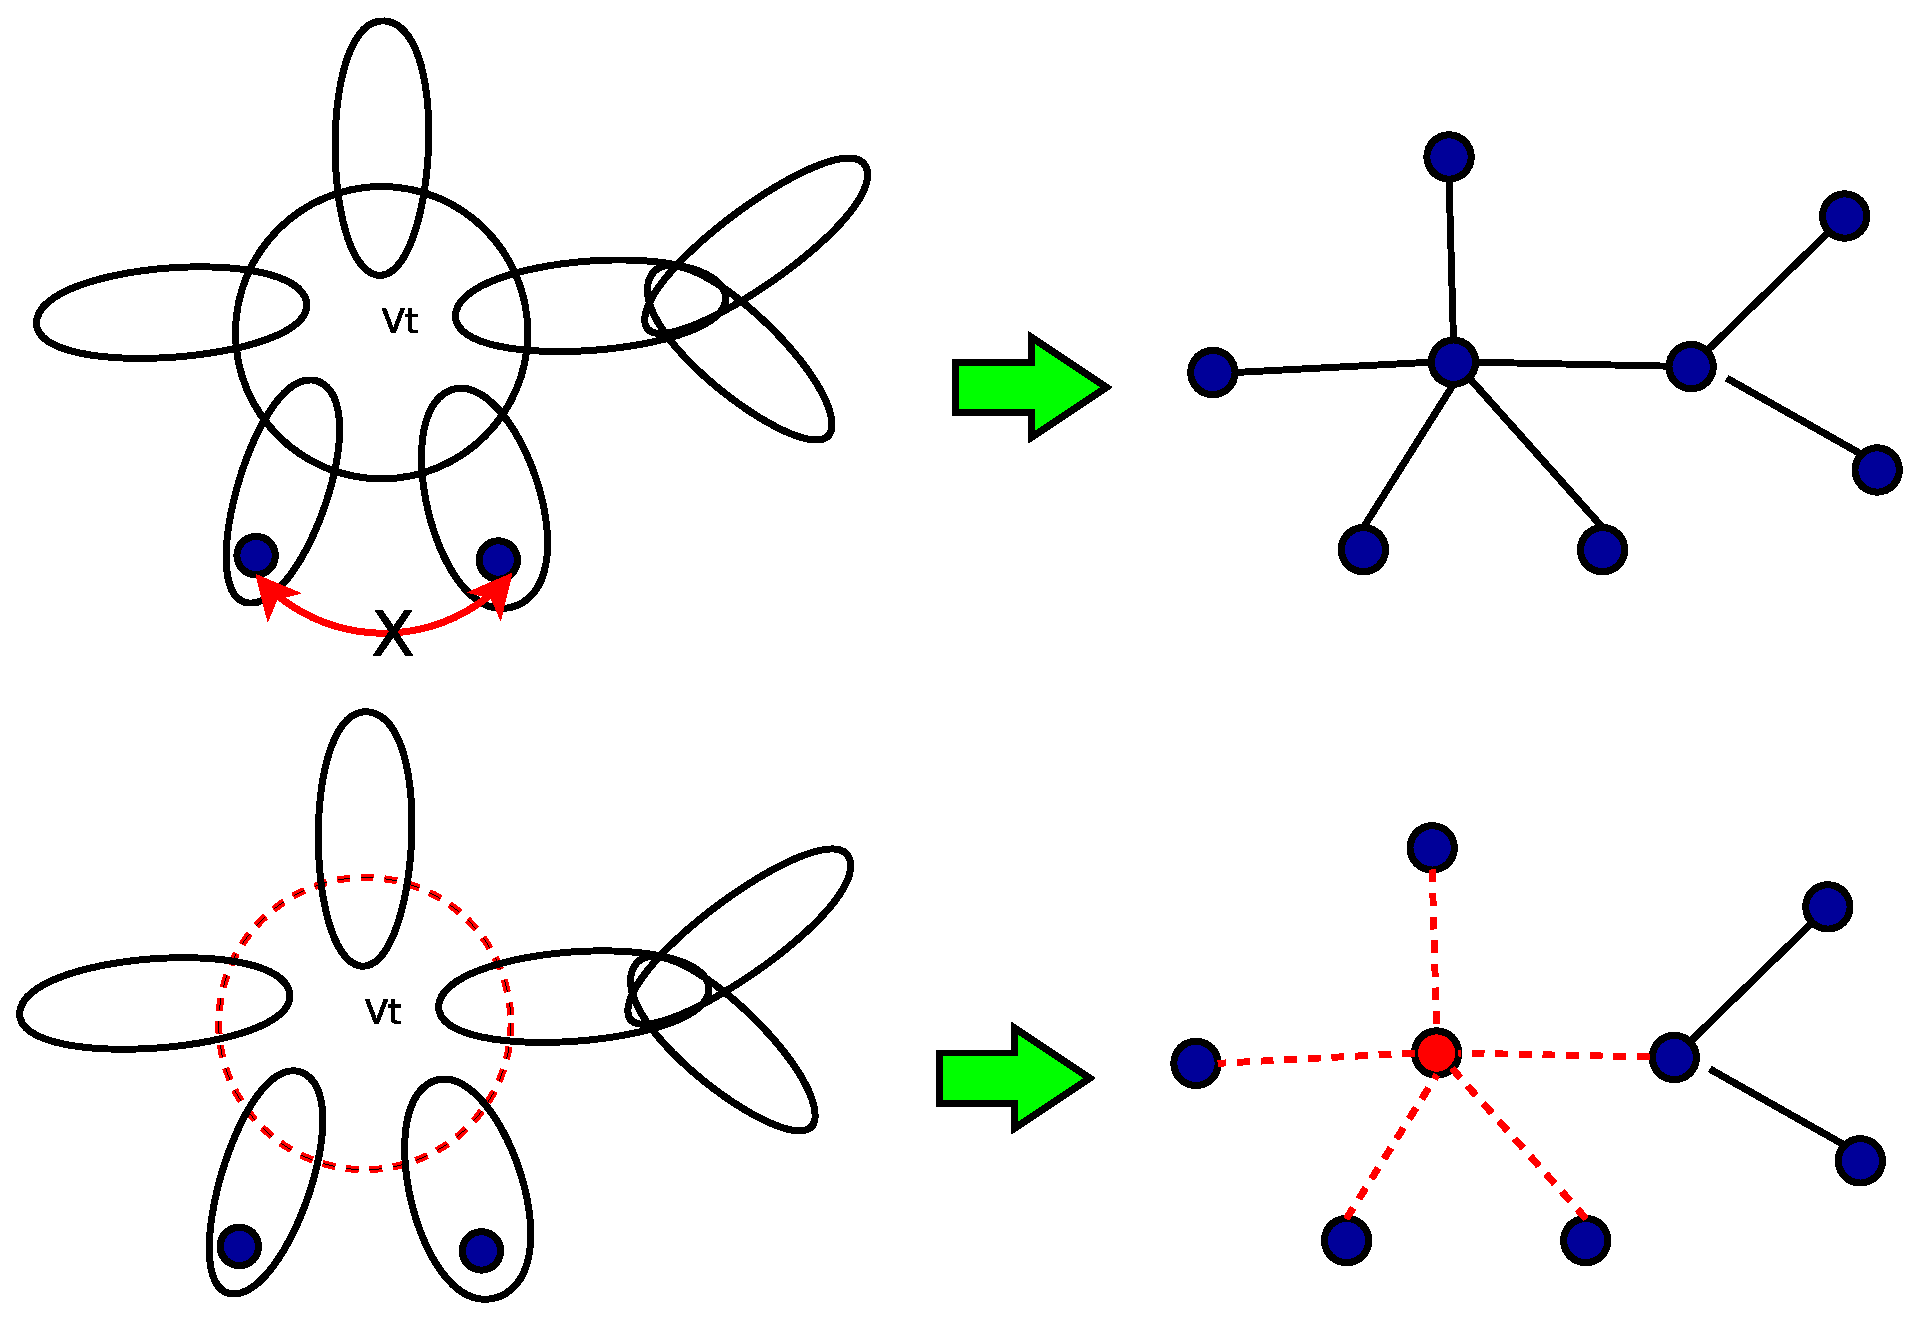
\includegraphics[width=3in] {L13-treedecompositionremovenode.eps}
\end{figure}
} 

\frame{
\frametitle{Removing an edge: generating independent sub-problems }

\begin{Theorem}
(Removing an edge) Suppose $T-\{e\}$ has two branches, namely $X$ and $Y$. Correspondingly, $G-\{V_x\cap V_y\}$ has two subgraphs: $G_X-\{V_X\cap V_y\}$, and $G_Y -\{V_X\cap V_Y\}$. The two subgraphs share no common nodes and no edge can connect them. 
\end{Theorem}
%(Intuition: removing an edge of $T$ also results in the decompostion of $G$.)
\begin{figure}
 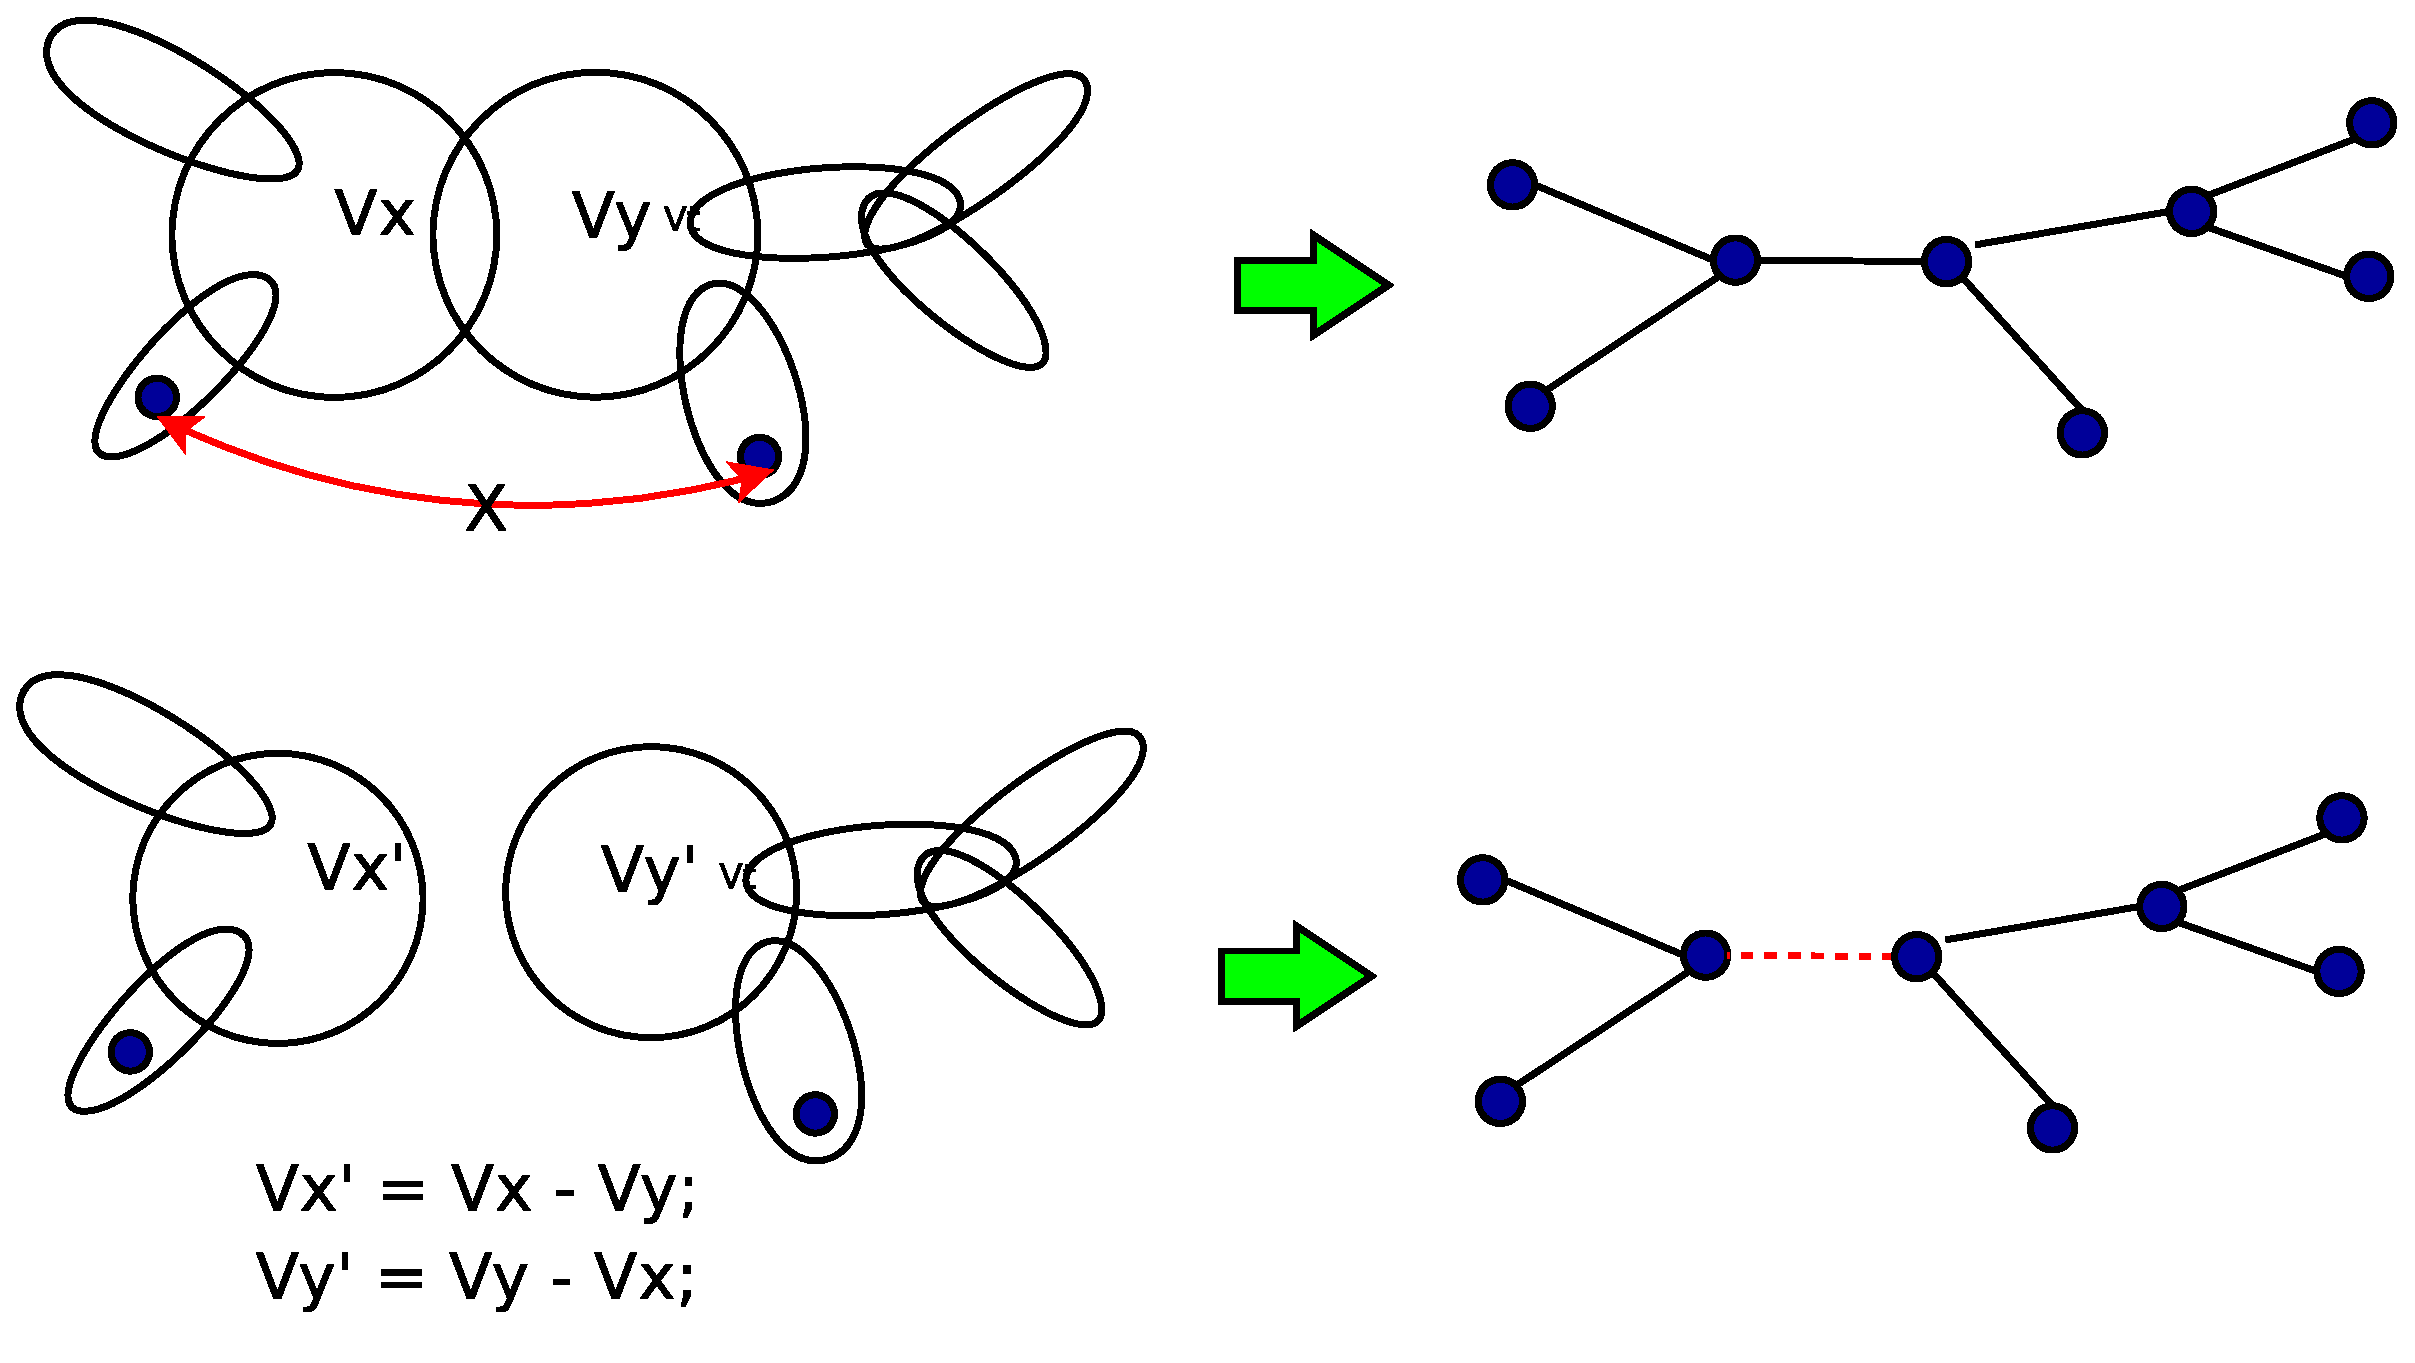
\includegraphics[width=3.5in] {L13-treedecompositionremoveedge.eps}
\end{figure}
}


\frame{
\frametitle{ Tree-width: an intrinsic property of a graph }
\begin{itemize}
 \item Every graph $G$ has a tree-composition. (A trivial tree-decomposition: $T$ has only one node $t$, and $V_t=V$. (See an extra slide)
 \item We are interested in the tree-composition with \textcolor{red}{small pieces}. (Intuition: removal of a piece will break the graph into INDEPENDENT parts. )
\end{itemize}
\begin{definition}[Tree-Width]
 $TreeWidth(G)=\max_t |V_t| - 1 $. 
\end{definition}
Note: Why $-1$? Just to make the tree-width of a tree be $1$. 
} 

\frame{
\frametitle{ An example: tree-decomposition of a tree  }

\begin{itemize}
 \item Tree-decomposition of a tree $G=(V,E)$:
 	\begin{itemize}
	\item For each node $u\in V$, create a piece $V_u$, and for each edge $e$, create a piece $V_e$. 
	\item  Connecting two pieces if they share a common node. 
	\item Verify the three requirements and $TreeWidth(G)=1$.  
	\end{itemize} 
\end{itemize}
\begin{figure}
 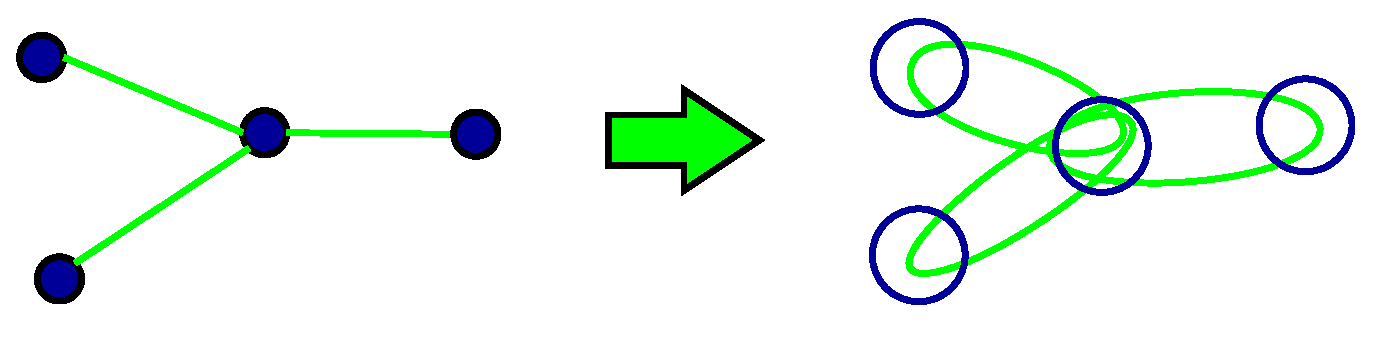
\includegraphics[width=3in] {L13-treedecompositiontree.eps}
\end{figure}
}

\frame[allowframebreaks]{
\frametitle{}
\begin{Theorem}
  A connected graph $G$ has a width of $1$ iff $G$ is a tree. 
\end{Theorem}
\begin{Proof} 
\begin{small}
 \begin{itemize}
\item Suppose $G$ is not a tree but $width(G)=1$. 
\item There is  a cycle $C$ in $G$. Consider two edges $e=(u,v)$ and $e'=(u',v')$. The corresponding pieces are denoted as $V_e$ and $V_{e'}$. 
\item There should be a path connecting $V_e$ and $V_{e'}$ in $T$. (by the connection property of tree.)
\item Consider a path $(x,y)$ in the path, and $V_x \neq V_y$. Thus $V_x \cap V_y \leq 1 $. 
\item Thus the removal of $V_x \cap V_y$ will decompose $C$ into two INDEPENDENT parts. (by the previous Theorem)
\item However, we cannot decompose a cycle into two INDEPENDENT part through removing ONLY one edge. 
 \end{itemize}
 \end{small}
\end{Proof}
 \begin{small}
 Fact: Suppose $H$ is a subgraph of $G$. We have $width(H)\leq width(G)$. (Argument: constructing $T_H$ based on $T_G$: $V_t^H = V_t^G \cap H$. Verify the three requirements.)
 \end{small}
}

\frame{
	\begin{block}
		Finding maximum independent set in a general graph
	\end{block}
	
}




\frame[allowframebreaks]{
\frametitle{Finding maximum independent set in a general graph}
\begin{itemize}
 
 \item Basic idea: 
 	\begin{itemize} 
		\item  For a general graph $G=(V,E)$, we construct its tree-decomposition $T$ first. 
		\item Let's travel $T$ in the bottom-up manner
		\item  Consider  node $t$ of tree $T$. The maximum independent set intersects the piece $V_t$ onto a subset $U$. 
		\item However, we have no idea what nodes that $U$ has.
		\item  Solution: enumerate all possibility of $U$ within $V_t$. This operation costs at most $2^{w+1}$ time. 
		\item The properties of $T$ ensure that the sub-problems corresponding to sub-trees of $t$ can be INDEPENDENTLY solved as soon as $U$ is determined.
	\end{itemize} 

\begin{figure}
 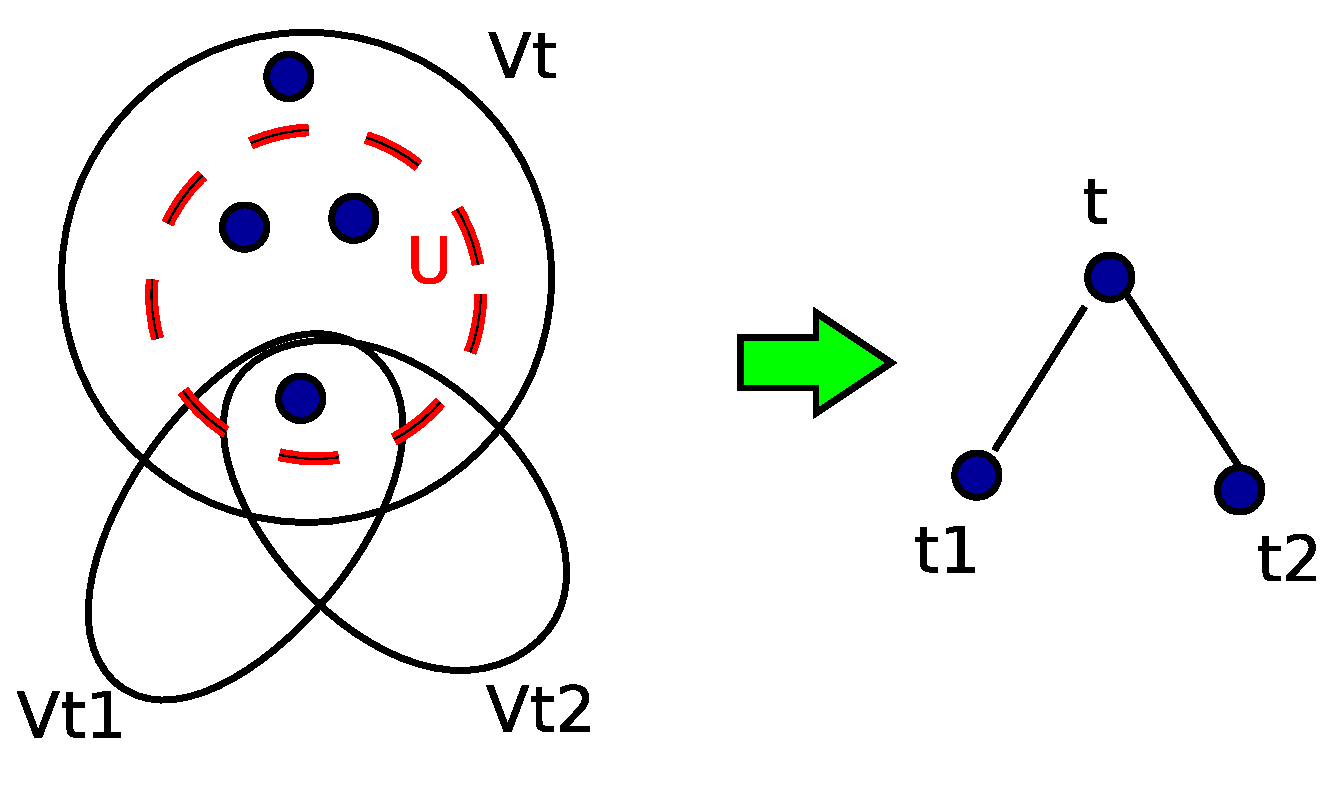
\includegraphics[width=3in] {L13-treedecompositionDP.eps}
\end{figure}


\item Key observation: (sub-problem) For each sub-tree $T_t$, we define a FAMILY of sub-problems: for each subset $U\in V_t$, we use $f_t(U)$ to denote the value of the maximum independent set in $G_t$, where $U$ is an independent set. 


\item Optimal substructure: $f_t(U) = w(U)+ \sum_{i=1}^d \max\{ f_{t_i}(U_i) - w( U_i \cap U) \}$, where $U_i \cap V_t = U \cap V_{t_i}$ and $U_i \subset V_{t_i}$ is an independent set. 

\begin{figure}
 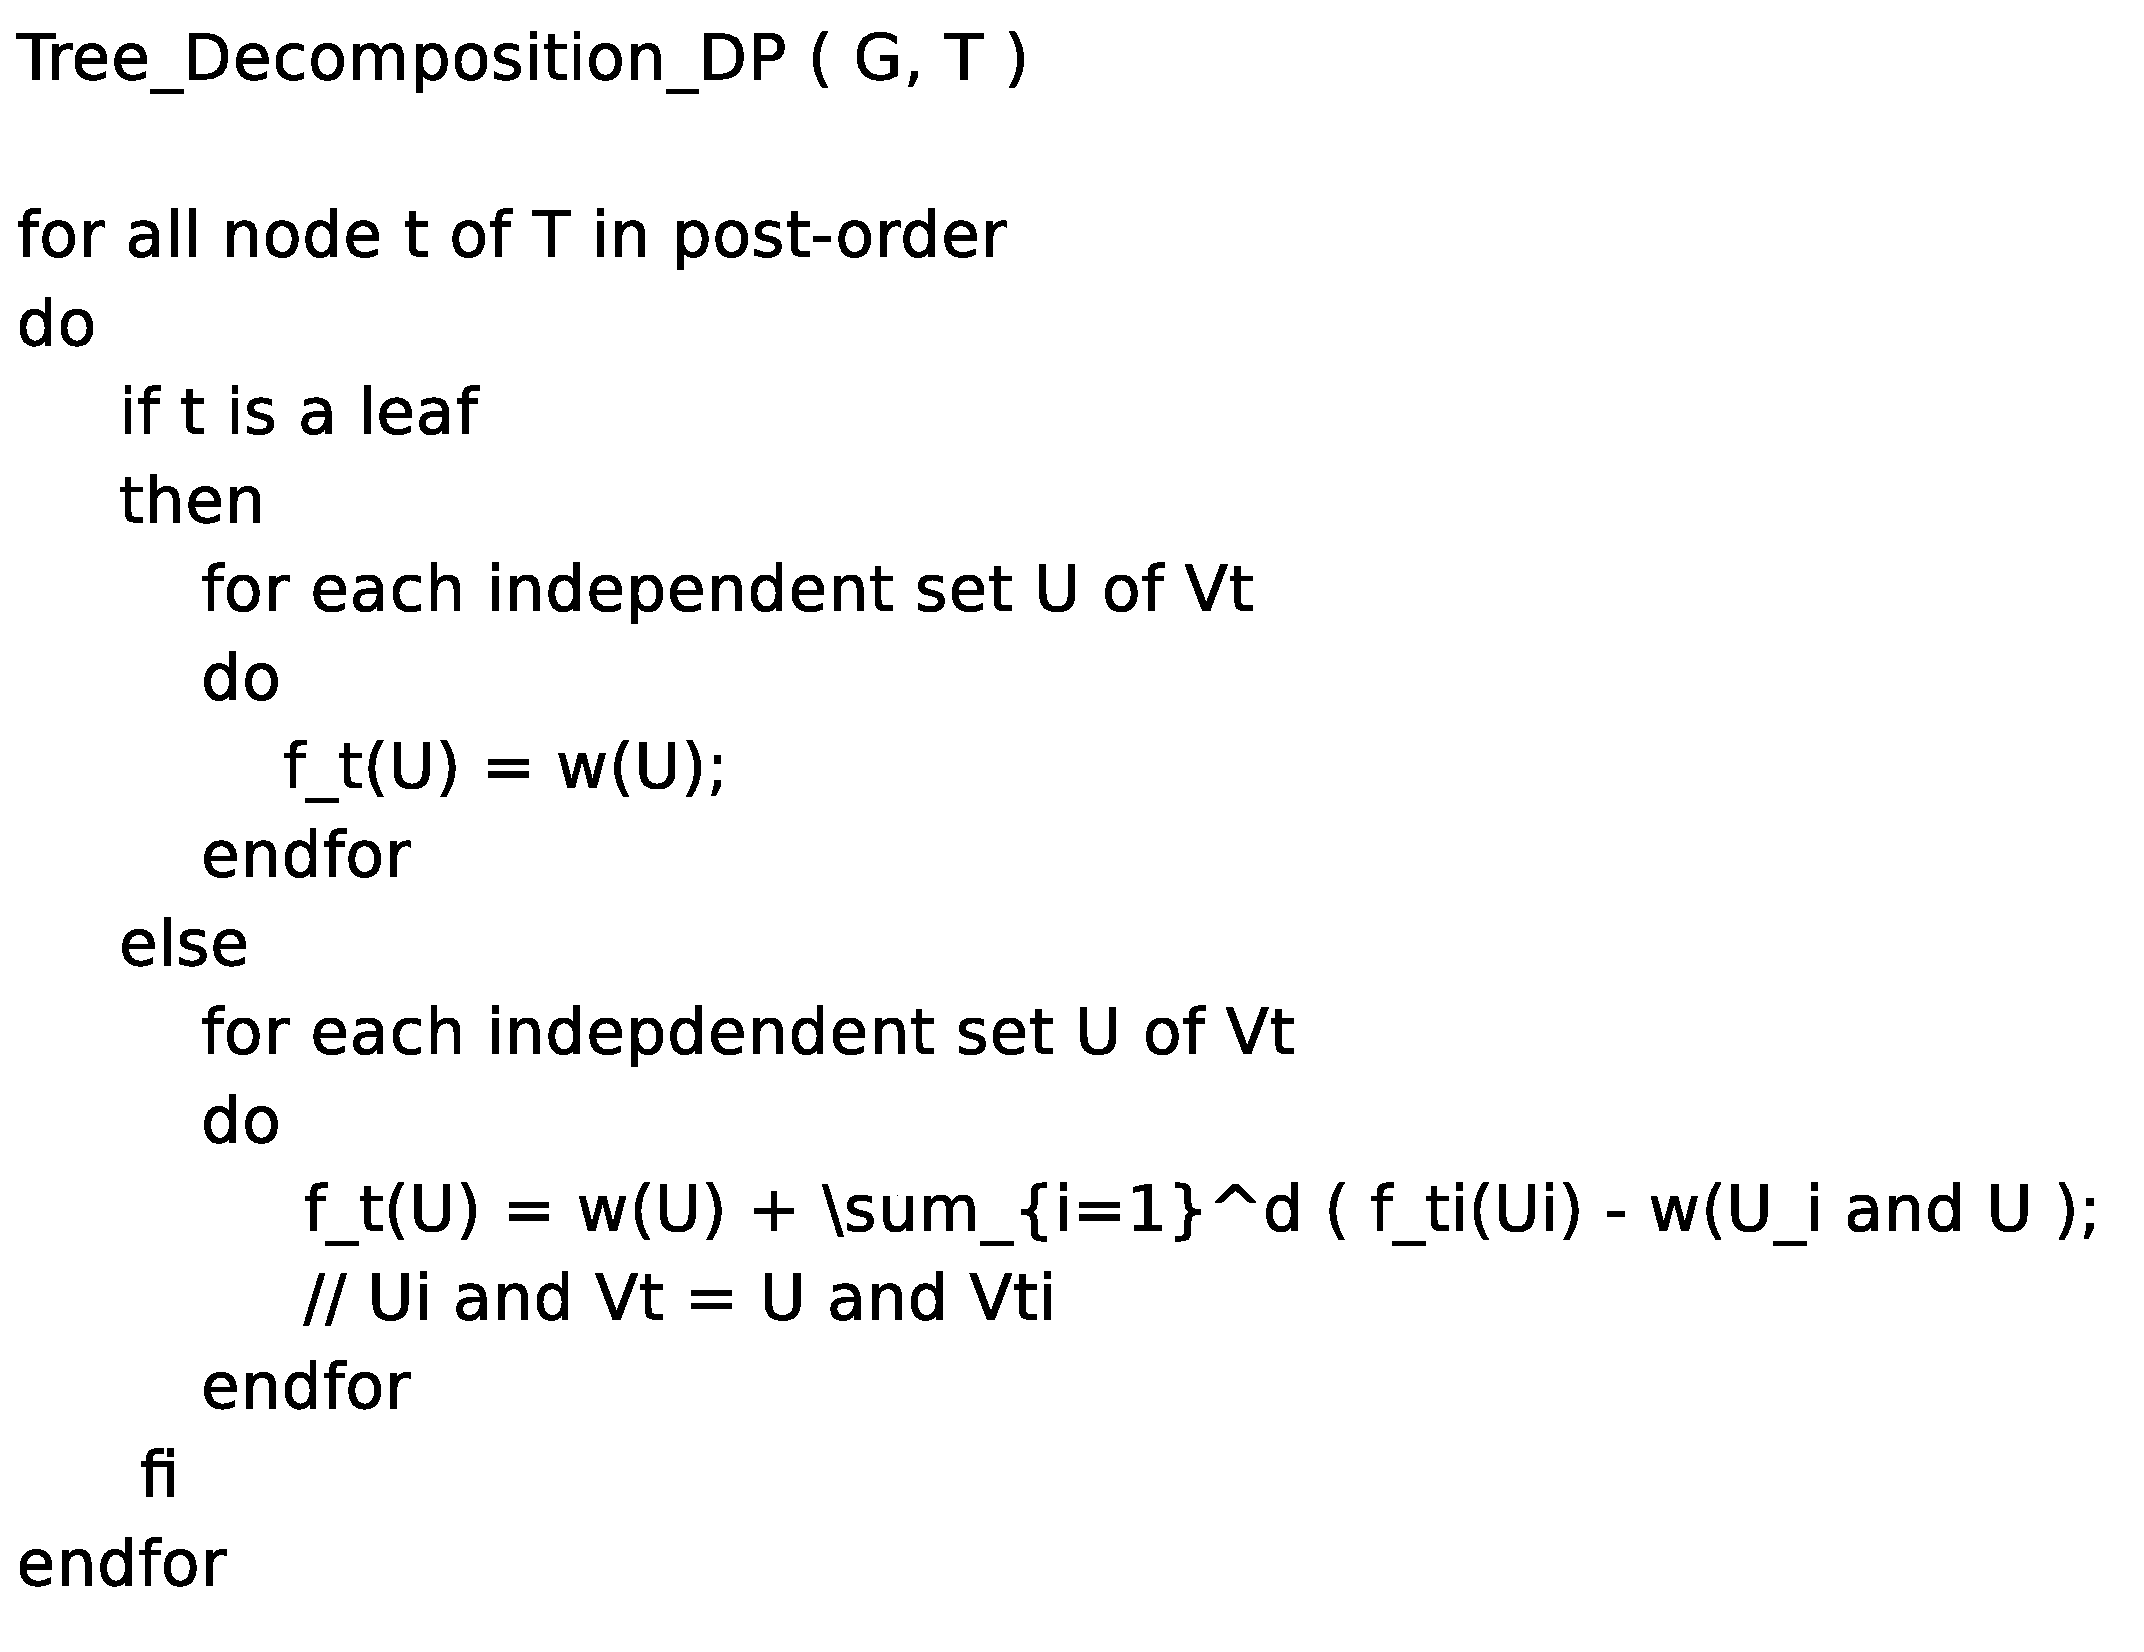
\includegraphics[width=3in] {L13-treedecompositionDPalgo.eps}
\end{figure}

\item Time-complexity: $O(2^w w n)$. 
\item Note: the practical graph, say network and residue contact map, usually have small width.
\end{itemize}

}


\end{document}
